%! TEX encoding = utf8
\chapter{Laboratorium}

\section{Określenie wartości pomiaru temperatury w punkcie pracy}

W celu określenia wartości pomiaru temperatury w punkcie pracy ustawiono moc wentylatora  $W1 = 50\%$,a moc grzałki $G1 = 25\%$.
Po czasie około 5 minut temperatura odczytywana przez czujnik temperatury zaczeła się stabilizować  na poziomie  $T1 = 28,4^{\circ} C$. 
Niestety z powodu ciągłego ruchu powietrza związanego z przemieszczaniem się osób w sali i dużej ilości tych osób wpływających na temperaturę sali oraz czułość stanowiska pomiarowego temperatura odczytywana przez czujnik zaczeła odbiegać i lekko oscylować wokół tej temperatury.

\begin{figure}[H]
\centering
% This file was created by matlab2tikz.
%
%The latest updates can be retrieved from
%  http://www.mathworks.com/matlabcentral/fileexchange/22022-matlab2tikz-matlab2tikz
%where you can also make suggestions and rate matlab2tikz.
%
\definecolor{mycolor1}{rgb}{0.00000,0.44700,0.74100}%
%
\begin{tikzpicture}

\begin{axis}[%
width=4.521in,
height=3.566in,
at={(0.758in,0.481in)},
scale only axis,
xmin=0,
xmax=400,
xlabel style={font=\color{white!15!black}},
xlabel={k},
ymin=21,
ymax=29,
ylabel style={font=\color{white!15!black}},
ylabel={$\text{T[}^\circ\text{C]}$},
axis background/.style={fill=white}
]
\addplot[const plot, color=mycolor1, forget plot] table[row sep=crcr] {%
1	21.12\\
2	21.12\\
3	21.12\\
4	21.06\\
5	21.06\\
6	21.06\\
7	21.06\\
8	21.12\\
9	21.12\\
10	21.12\\
11	21.12\\
12	21.18\\
13	21.18\\
14	21.18\\
15	21.25\\
16	21.31\\
17	21.31\\
18	21.37\\
19	21.43\\
20	21.56\\
21	21.56\\
22	21.62\\
23	21.68\\
24	21.75\\
25	21.87\\
26	21.93\\
27	22\\
28	22.06\\
29	22.12\\
30	22.18\\
31	22.31\\
32	22.37\\
33	22.43\\
34	22.5\\
35	22.62\\
36	22.68\\
37	22.75\\
38	22.81\\
39	22.93\\
40	23\\
41	23.06\\
42	23.12\\
43	23.18\\
44	23.25\\
45	23.31\\
46	23.43\\
47	23.5\\
48	23.56\\
49	23.62\\
50	23.68\\
51	23.75\\
52	23.81\\
53	23.87\\
54	23.93\\
55	24\\
56	24.06\\
57	24.12\\
58	24.18\\
59	24.25\\
60	24.31\\
61	24.37\\
62	24.43\\
63	24.43\\
64	24.5\\
65	24.56\\
66	24.62\\
67	24.68\\
68	24.75\\
69	24.75\\
70	24.81\\
71	24.87\\
72	24.93\\
73	25\\
74	25\\
75	25.06\\
76	25.06\\
77	25.12\\
78	25.18\\
79	25.25\\
80	25.25\\
81	25.31\\
82	25.31\\
83	25.37\\
84	25.43\\
85	25.43\\
86	25.5\\
87	25.56\\
88	25.56\\
89	25.62\\
90	25.68\\
91	25.68\\
92	25.75\\
93	25.75\\
94	25.81\\
95	25.81\\
96	25.81\\
97	25.87\\
98	25.87\\
99	25.93\\
100	25.93\\
101	26\\
102	26\\
103	26.06\\
104	26.06\\
105	26.12\\
106	26.12\\
107	26.18\\
108	26.18\\
109	26.18\\
110	26.25\\
111	26.25\\
112	26.31\\
113	26.31\\
114	26.31\\
115	26.37\\
116	26.37\\
117	26.37\\
118	26.37\\
119	26.43\\
120	26.43\\
121	26.43\\
122	26.5\\
123	26.5\\
124	26.5\\
125	26.5\\
126	26.5\\
127	26.56\\
128	26.56\\
129	26.62\\
130	26.62\\
131	26.68\\
132	26.68\\
133	26.68\\
134	26.75\\
135	26.75\\
136	26.81\\
137	26.81\\
138	26.81\\
139	26.81\\
140	26.87\\
141	26.93\\
142	26.93\\
143	26.93\\
144	26.93\\
145	26.93\\
146	27\\
147	27\\
148	27.06\\
149	27.06\\
150	27.06\\
151	27.12\\
152	27.12\\
153	27.18\\
154	27.18\\
155	27.18\\
156	27.18\\
157	27.25\\
158	27.25\\
159	27.25\\
160	27.31\\
161	27.31\\
162	27.31\\
163	27.37\\
164	27.37\\
165	27.37\\
166	27.37\\
167	27.37\\
168	27.43\\
169	27.43\\
170	27.43\\
171	27.5\\
172	27.5\\
173	27.5\\
174	27.5\\
175	27.5\\
176	27.56\\
177	27.56\\
178	27.56\\
179	27.56\\
180	27.56\\
181	27.56\\
182	27.62\\
183	27.62\\
184	27.62\\
185	27.62\\
186	27.62\\
187	27.62\\
188	27.62\\
189	27.62\\
190	27.62\\
191	27.68\\
192	27.68\\
193	27.68\\
194	27.68\\
195	27.68\\
196	27.68\\
197	27.75\\
198	27.68\\
199	27.68\\
200	27.68\\
201	27.75\\
202	27.75\\
203	27.75\\
204	27.75\\
205	27.75\\
206	27.75\\
207	27.75\\
208	27.75\\
209	27.81\\
210	27.81\\
211	27.81\\
212	27.81\\
213	27.81\\
214	27.81\\
215	27.87\\
216	27.87\\
217	27.87\\
218	27.87\\
219	27.87\\
220	27.87\\
221	27.87\\
222	27.87\\
223	27.93\\
224	27.93\\
225	27.93\\
226	28\\
227	28\\
228	28\\
229	28\\
230	28.06\\
231	28.06\\
232	28.06\\
233	28.12\\
234	28.12\\
235	28.12\\
236	28.12\\
237	28.12\\
238	28.12\\
239	28.12\\
240	28.12\\
241	28.06\\
242	28.12\\
243	28.12\\
244	28.06\\
245	28.12\\
246	28.06\\
247	28.06\\
248	28.06\\
249	28.06\\
250	28.06\\
251	28.06\\
252	28.06\\
253	28.06\\
254	28.06\\
255	28.06\\
256	28.06\\
257	28.06\\
258	28.06\\
259	28.12\\
260	28.12\\
261	28.12\\
262	28.18\\
263	28.18\\
264	28.18\\
265	28.18\\
266	28.25\\
267	28.25\\
268	28.25\\
269	28.25\\
270	28.25\\
271	28.25\\
272	28.25\\
273	28.25\\
274	28.25\\
275	28.25\\
276	28.25\\
277	28.25\\
278	28.25\\
279	28.25\\
280	28.25\\
281	28.25\\
282	28.25\\
283	28.25\\
284	28.25\\
285	28.25\\
286	28.25\\
287	28.25\\
288	28.25\\
289	28.25\\
290	28.25\\
291	28.25\\
292	28.31\\
293	28.31\\
294	28.31\\
295	28.31\\
296	28.31\\
297	28.31\\
298	28.37\\
299	28.37\\
300	28.37\\
301	28.31\\
302	28.37\\
303	28.31\\
304	28.31\\
305	28.31\\
306	28.31\\
307	28.37\\
308	28.37\\
309	28.37\\
310	28.37\\
311	28.43\\
312	28.43\\
313	28.43\\
314	28.43\\
315	28.43\\
316	28.43\\
317	28.43\\
318	28.43\\
319	28.43\\
320	28.43\\
321	28.43\\
322	28.43\\
323	28.43\\
324	28.43\\
325	28.43\\
326	28.43\\
327	28.43\\
328	28.43\\
329	28.43\\
330	28.43\\
331	28.43\\
332	28.43\\
333	28.37\\
334	28.37\\
335	28.43\\
336	28.43\\
337	28.37\\
338	28.43\\
339	28.43\\
340	28.43\\
341	28.43\\
342	28.43\\
343	28.43\\
344	28.5\\
345	28.43\\
346	28.43\\
347	28.43\\
348	28.5\\
349	28.5\\
350	28.5\\
351	28.5\\
352	28.5\\
353	28.5\\
354	28.5\\
355	28.5\\
356	28.5\\
357	28.5\\
358	28.5\\
359	28.5\\
360	28.5\\
361	28.5\\
362	28.5\\
363	28.56\\
364	28.5\\
365	28.56\\
366	28.56\\
367	28.56\\
368	28.5\\
369	28.5\\
370	28.5\\
371	28.5\\
372	28.5\\
373	28.5\\
374	28.5\\
375	28.5\\
376	28.5\\
377	28.5\\
378	28.56\\
379	28.56\\
380	28.56\\
381	28.62\\
382	28.62\\
383	28.62\\
384	28.68\\
385	28.68\\
386	28.62\\
387	28.68\\
388	28.68\\
389	28.68\\
390	28.68\\
391	28.68\\
392	28.68\\
393	28.68\\
394	28.68\\
395	28.68\\
396	28.68\\
397	28.68\\
398	28.68\\
399	28.68\\
400	28.68\\
};
\end{axis}
\end{tikzpicture}%
\caption{Pomiar temperatury w punkcie pracy}
\end{figure}

\section{Wyznaczenie odpowiedzi skokowych}

Rozpoczynając z punktu pracy wyznaczono odpowiedzi skokowe dla trzech różnych wartości sygnału sterującego  $G1 = 35\%$  $G1 = 45\%$ i $G1 = 55\%$.

\begin{figure}[H]
\centering
% This file was created by matlab2tikz.
%
%The latest updates can be retrieved from
%  http://www.mathworks.com/matlabcentral/fileexchange/22022-matlab2tikz-matlab2tikz
%where you can also make suggestions and rate matlab2tikz.
%
\definecolor{mycolor1}{rgb}{0.00000,0.44700,0.74100}%
\definecolor{mycolor2}{rgb}{0.85000,0.32500,0.09800}%
\definecolor{mycolor3}{rgb}{0.92900,0.69400,0.12500}%
%
\begin{tikzpicture}

\begin{axis}[%
width=4.521in,
height=3.566in,
at={(0.758in,0.481in)},
scale only axis,
xmin=0,
xmax=350,
xlabel style={font=\color{white!15!black}},
xlabel={k},
ymin=28,
ymax=40,
ylabel style={font=\color{white!15!black}},
ylabel={$\text{T[}^\circ\text{C]}$},
axis background/.style={fill=white}
]
\addplot[const plot, color=mycolor1, forget plot] table[row sep=crcr] {%
1	28.5\\
2	28.5\\
3	28.56\\
4	28.56\\
5	28.56\\
6	28.5\\
7	28.5\\
8	28.5\\
9	28.5\\
10	28.5\\
11	28.5\\
12	28.5\\
13	28.5\\
14	28.5\\
15	28.5\\
16	28.5\\
17	28.43\\
18	28.43\\
19	28.43\\
20	28.43\\
21	28.43\\
22	28.43\\
23	28.43\\
24	28.43\\
25	28.43\\
26	28.43\\
27	28.43\\
28	28.43\\
29	28.5\\
30	28.5\\
31	28.56\\
32	28.56\\
33	28.56\\
34	28.62\\
35	28.62\\
36	28.62\\
37	28.68\\
38	28.68\\
39	28.68\\
40	28.68\\
41	28.75\\
42	28.75\\
43	28.75\\
44	28.81\\
45	28.87\\
46	28.87\\
47	28.87\\
48	28.93\\
49	28.93\\
50	29\\
51	29\\
52	29.06\\
53	29.06\\
54	29.12\\
55	29.18\\
56	29.25\\
57	29.25\\
58	29.25\\
59	29.31\\
60	29.37\\
61	29.37\\
62	29.37\\
63	29.43\\
64	29.5\\
65	29.5\\
66	29.56\\
67	29.62\\
68	29.62\\
69	29.68\\
70	29.68\\
71	29.68\\
72	29.75\\
73	29.75\\
74	29.81\\
75	29.81\\
76	29.81\\
77	29.87\\
78	29.87\\
79	29.93\\
80	29.93\\
81	29.93\\
82	29.93\\
83	30\\
84	30\\
85	30\\
86	30.06\\
87	30.06\\
88	30.06\\
89	30.12\\
90	30.12\\
91	30.12\\
92	30.18\\
93	30.18\\
94	30.18\\
95	30.18\\
96	30.18\\
97	30.25\\
98	30.25\\
99	30.25\\
100	30.25\\
101	30.31\\
102	30.31\\
103	30.31\\
104	30.37\\
105	30.37\\
106	30.37\\
107	30.37\\
108	30.37\\
109	30.43\\
110	30.43\\
111	30.43\\
112	30.5\\
113	30.5\\
114	30.5\\
115	30.5\\
116	30.56\\
117	30.56\\
118	30.62\\
119	30.62\\
120	30.62\\
121	30.68\\
122	30.68\\
123	30.68\\
124	30.68\\
125	30.68\\
126	30.68\\
127	30.68\\
128	30.75\\
129	30.75\\
130	30.75\\
131	30.75\\
132	30.75\\
133	30.75\\
134	30.75\\
135	30.81\\
136	30.81\\
137	30.81\\
138	30.87\\
139	30.87\\
140	30.87\\
141	30.87\\
142	30.93\\
143	30.93\\
144	30.93\\
145	31\\
146	31\\
147	31\\
148	31\\
149	31.06\\
150	31.06\\
151	31.06\\
152	31.06\\
153	31.06\\
154	31.06\\
155	31.12\\
156	31.12\\
157	31.12\\
158	31.12\\
159	31.12\\
160	31.12\\
161	31.12\\
162	31.12\\
163	31.12\\
164	31.12\\
165	31.18\\
166	31.18\\
167	31.18\\
168	31.18\\
169	31.18\\
170	31.18\\
171	31.18\\
172	31.18\\
173	31.18\\
174	31.18\\
175	31.18\\
176	31.18\\
177	31.25\\
178	31.25\\
179	31.25\\
180	31.25\\
181	31.25\\
182	31.25\\
183	31.25\\
184	31.25\\
185	31.25\\
186	31.25\\
187	31.25\\
188	31.25\\
189	31.18\\
190	31.18\\
191	31.18\\
192	31.25\\
193	31.18\\
194	31.25\\
195	31.25\\
196	31.25\\
197	31.25\\
198	31.25\\
199	31.25\\
200	31.25\\
201	31.25\\
202	31.25\\
203	31.25\\
204	31.25\\
205	31.25\\
206	31.25\\
207	31.25\\
208	31.25\\
209	31.25\\
210	31.25\\
211	31.25\\
212	31.31\\
213	31.31\\
214	31.31\\
215	31.31\\
216	31.31\\
217	31.37\\
218	31.37\\
219	31.37\\
220	31.37\\
221	31.37\\
222	31.43\\
223	31.43\\
224	31.43\\
225	31.43\\
226	31.37\\
227	31.37\\
228	31.37\\
229	31.37\\
230	31.37\\
231	31.37\\
232	31.37\\
233	31.37\\
234	31.37\\
235	31.37\\
236	31.37\\
237	31.37\\
238	31.37\\
239	31.43\\
240	31.43\\
241	31.43\\
242	31.43\\
243	31.43\\
244	31.43\\
245	31.43\\
246	31.43\\
247	31.43\\
248	31.43\\
249	31.43\\
250	31.43\\
251	31.43\\
252	31.43\\
253	31.43\\
254	31.43\\
255	31.5\\
256	31.43\\
257	31.43\\
258	31.5\\
259	31.5\\
260	31.5\\
261	31.5\\
262	31.5\\
263	31.5\\
264	31.5\\
265	31.5\\
266	31.43\\
267	31.5\\
268	31.5\\
269	31.5\\
270	31.43\\
271	31.5\\
272	31.43\\
273	31.43\\
274	31.43\\
275	31.43\\
276	31.43\\
277	31.43\\
278	31.43\\
279	31.43\\
280	31.43\\
281	31.43\\
282	31.43\\
283	31.43\\
284	31.43\\
285	31.43\\
286	31.43\\
287	31.43\\
288	31.43\\
289	31.37\\
290	31.37\\
291	31.43\\
292	31.43\\
293	31.43\\
294	31.43\\
295	31.43\\
296	31.43\\
297	31.43\\
298	31.43\\
299	31.43\\
300	31.43\\
301	31.43\\
302	31.43\\
303	31.43\\
304	31.43\\
305	31.43\\
306	31.43\\
307	31.43\\
308	31.5\\
309	31.5\\
310	31.5\\
311	31.5\\
312	31.56\\
313	31.56\\
314	31.56\\
315	31.56\\
316	31.56\\
317	31.56\\
318	31.56\\
319	31.56\\
320	31.56\\
321	31.56\\
322	31.62\\
323	31.56\\
324	31.56\\
325	31.56\\
326	31.56\\
327	31.56\\
328	31.56\\
329	31.56\\
330	31.56\\
331	31.56\\
332	31.56\\
333	31.56\\
334	31.56\\
335	31.56\\
336	31.56\\
337	31.56\\
338	31.56\\
339	31.56\\
340	31.56\\
341	31.62\\
342	31.62\\
343	31.62\\
344	31.62\\
345	31.62\\
346	31.62\\
347	31.62\\
348	31.62\\
349	31.62\\
350	31.56\\
};
\addplot[const plot, color=mycolor2, forget plot] table[row sep=crcr] {%
1	28.56\\
2	28.56\\
3	28.59\\
4	28.59\\
5	28.59\\
6	28.56\\
7	28.59\\
8	28.59\\
9	28.59\\
10	28.59\\
11	28.59\\
12	28.59\\
13	28.59\\
14	28.59\\
15	28.59\\
16	28.59\\
17	28.555\\
18	28.555\\
19	28.555\\
20	28.555\\
21	28.555\\
22	28.59\\
23	28.59\\
24	28.59\\
25	28.59\\
26	28.62\\
27	28.62\\
28	28.62\\
29	28.655\\
30	28.685\\
31	28.715\\
32	28.745\\
33	28.78\\
34	28.81\\
35	28.84\\
36	28.87\\
37	28.93\\
38	28.965\\
39	28.995\\
40	29.055\\
41	29.125\\
42	29.185\\
43	29.215\\
44	29.31\\
45	29.37\\
46	29.435\\
47	29.465\\
48	29.555\\
49	29.59\\
50	29.685\\
51	29.715\\
52	29.81\\
53	29.84\\
54	29.935\\
55	29.995\\
56	30.09\\
57	30.125\\
58	30.185\\
59	30.245\\
60	30.34\\
61	30.37\\
62	30.435\\
63	30.525\\
64	30.59\\
65	30.625\\
66	30.715\\
67	30.775\\
68	30.84\\
69	30.9\\
70	30.965\\
71	30.995\\
72	31.06\\
73	31.125\\
74	31.185\\
75	31.215\\
76	31.245\\
77	31.31\\
78	31.34\\
79	31.4\\
80	31.43\\
81	31.465\\
82	31.495\\
83	31.59\\
84	31.625\\
85	31.655\\
86	31.715\\
87	31.745\\
88	31.78\\
89	31.84\\
90	31.87\\
91	31.9\\
92	31.965\\
93	31.995\\
94	32.025\\
95	32.055\\
96	32.09\\
97	32.155\\
98	32.185\\
99	32.215\\
100	32.25\\
101	32.28\\
102	32.34\\
103	32.34\\
104	32.4\\
105	32.435\\
106	32.465\\
107	32.525\\
108	32.525\\
109	32.59\\
110	32.62\\
111	32.62\\
112	32.715\\
113	32.715\\
114	32.75\\
115	32.75\\
116	32.81\\
117	32.84\\
118	32.87\\
119	32.87\\
120	32.9\\
121	32.965\\
122	32.965\\
123	32.965\\
124	32.965\\
125	32.995\\
126	32.995\\
127	33.025\\
128	33.06\\
129	33.09\\
130	33.125\\
131	33.125\\
132	33.155\\
133	33.185\\
134	33.185\\
135	33.245\\
136	33.28\\
137	33.28\\
138	33.34\\
139	33.34\\
140	33.37\\
141	33.37\\
142	33.4\\
143	33.43\\
144	33.43\\
145	33.465\\
146	33.465\\
147	33.5\\
148	33.5\\
149	33.53\\
150	33.53\\
151	33.56\\
152	33.56\\
153	33.56\\
154	33.59\\
155	33.65\\
156	33.65\\
157	33.65\\
158	33.65\\
159	33.685\\
160	33.685\\
161	33.685\\
162	33.715\\
163	33.715\\
164	33.715\\
165	33.775\\
166	33.775\\
167	33.805\\
168	33.805\\
169	33.84\\
170	33.87\\
171	33.87\\
172	33.9\\
173	33.93\\
174	33.93\\
175	33.93\\
176	33.965\\
177	34\\
178	34\\
179	34\\
180	34\\
181	34\\
182	34\\
183	34\\
184	34\\
185	34\\
186	34.03\\
187	34.06\\
188	34.06\\
189	34.055\\
190	34.09\\
191	34.09\\
192	34.125\\
193	34.12\\
194	34.155\\
195	34.125\\
196	34.125\\
197	34.125\\
198	34.125\\
199	34.125\\
200	34.125\\
201	34.125\\
202	34.155\\
203	34.155\\
204	34.155\\
205	34.185\\
206	34.215\\
207	34.215\\
208	34.215\\
209	34.25\\
210	34.25\\
211	34.28\\
212	34.31\\
213	34.31\\
214	34.34\\
215	34.34\\
216	34.37\\
217	34.4\\
218	34.435\\
219	34.435\\
220	34.465\\
221	34.465\\
222	34.495\\
223	34.495\\
224	34.495\\
225	34.495\\
226	34.465\\
227	34.465\\
228	34.495\\
229	34.495\\
230	34.495\\
231	34.525\\
232	34.525\\
233	34.525\\
234	34.525\\
235	34.525\\
236	34.525\\
237	34.525\\
238	34.525\\
239	34.555\\
240	34.555\\
241	34.555\\
242	34.555\\
243	34.555\\
244	34.555\\
245	34.555\\
246	34.525\\
247	34.555\\
248	34.555\\
249	34.525\\
250	34.555\\
251	34.555\\
252	34.555\\
253	34.59\\
254	34.62\\
255	34.655\\
256	34.65\\
257	34.68\\
258	34.715\\
259	34.75\\
260	34.75\\
261	34.78\\
262	34.78\\
263	34.78\\
264	34.78\\
265	34.78\\
266	34.745\\
267	34.78\\
268	34.78\\
269	34.78\\
270	34.775\\
271	34.81\\
272	34.775\\
273	34.775\\
274	34.775\\
275	34.775\\
276	34.775\\
277	34.775\\
278	34.775\\
279	34.805\\
280	34.805\\
281	34.84\\
282	34.84\\
283	34.84\\
284	34.84\\
285	34.84\\
286	34.84\\
287	34.84\\
288	34.805\\
289	34.775\\
290	34.775\\
291	34.775\\
292	34.775\\
293	34.775\\
294	34.745\\
295	34.745\\
296	34.745\\
297	34.745\\
298	34.745\\
299	34.745\\
300	34.775\\
301	34.745\\
302	34.745\\
303	34.745\\
304	34.745\\
305	34.775\\
306	34.775\\
307	34.805\\
308	34.84\\
309	34.84\\
310	34.84\\
311	34.84\\
312	34.87\\
313	34.87\\
314	34.87\\
315	34.905\\
316	34.905\\
317	34.905\\
318	34.935\\
319	34.905\\
320	34.935\\
321	34.935\\
322	34.965\\
323	34.935\\
324	34.965\\
325	34.965\\
326	34.995\\
327	34.995\\
328	34.995\\
329	35.03\\
330	35.03\\
331	35.03\\
332	35.06\\
333	35.06\\
334	35.06\\
335	35.03\\
336	35.03\\
337	35.06\\
338	35.03\\
339	35.06\\
340	35.06\\
341	35.09\\
342	35.06\\
343	35.06\\
344	35.06\\
345	35.025\\
346	35.025\\
347	34.995\\
348	34.995\\
349	34.995\\
350	34.935\\
};
\addplot[const plot, color=mycolor3, forget plot] table[row sep=crcr] {%
1	28.62\\
2	28.62\\
3	28.62\\
4	28.62\\
5	28.62\\
6	28.62\\
7	28.68\\
8	28.68\\
9	28.68\\
10	28.68\\
11	28.68\\
12	28.68\\
13	28.68\\
14	28.68\\
15	28.68\\
16	28.68\\
17	28.68\\
18	28.68\\
19	28.68\\
20	28.68\\
21	28.68\\
22	28.75\\
23	28.75\\
24	28.75\\
25	28.75\\
26	28.81\\
27	28.81\\
28	28.81\\
29	28.81\\
30	28.87\\
31	28.87\\
32	28.93\\
33	29\\
34	29\\
35	29.06\\
36	29.12\\
37	29.18\\
38	29.25\\
39	29.31\\
40	29.43\\
41	29.5\\
42	29.62\\
43	29.68\\
44	29.81\\
45	29.87\\
46	30\\
47	30.06\\
48	30.18\\
49	30.25\\
50	30.37\\
51	30.43\\
52	30.56\\
53	30.62\\
54	30.75\\
55	30.81\\
56	30.93\\
57	31\\
58	31.12\\
59	31.18\\
60	31.31\\
61	31.37\\
62	31.5\\
63	31.62\\
64	31.68\\
65	31.75\\
66	31.87\\
67	31.93\\
68	32.06\\
69	32.12\\
70	32.25\\
71	32.31\\
72	32.37\\
73	32.5\\
74	32.56\\
75	32.62\\
76	32.68\\
77	32.75\\
78	32.81\\
79	32.87\\
80	32.93\\
81	33\\
82	33.06\\
83	33.18\\
84	33.25\\
85	33.31\\
86	33.37\\
87	33.43\\
88	33.5\\
89	33.56\\
90	33.62\\
91	33.68\\
92	33.75\\
93	33.81\\
94	33.87\\
95	33.93\\
96	34\\
97	34.06\\
98	34.12\\
99	34.18\\
100	34.25\\
101	34.25\\
102	34.37\\
103	34.37\\
104	34.43\\
105	34.5\\
106	34.56\\
107	34.68\\
108	34.68\\
109	34.75\\
110	34.81\\
111	34.81\\
112	34.93\\
113	34.93\\
114	35\\
115	35\\
116	35.06\\
117	35.12\\
118	35.12\\
119	35.12\\
120	35.18\\
121	35.25\\
122	35.25\\
123	35.25\\
124	35.25\\
125	35.31\\
126	35.31\\
127	35.37\\
128	35.37\\
129	35.43\\
130	35.5\\
131	35.5\\
132	35.56\\
133	35.62\\
134	35.62\\
135	35.68\\
136	35.75\\
137	35.75\\
138	35.81\\
139	35.81\\
140	35.87\\
141	35.87\\
142	35.87\\
143	35.93\\
144	35.93\\
145	35.93\\
146	35.93\\
147	36\\
148	36\\
149	36\\
150	36\\
151	36.06\\
152	36.06\\
153	36.06\\
154	36.12\\
155	36.18\\
156	36.18\\
157	36.18\\
158	36.18\\
159	36.25\\
160	36.25\\
161	36.25\\
162	36.31\\
163	36.31\\
164	36.31\\
165	36.37\\
166	36.37\\
167	36.43\\
168	36.43\\
169	36.5\\
170	36.56\\
171	36.56\\
172	36.62\\
173	36.68\\
174	36.68\\
175	36.68\\
176	36.75\\
177	36.75\\
178	36.75\\
179	36.75\\
180	36.75\\
181	36.75\\
182	36.75\\
183	36.75\\
184	36.75\\
185	36.75\\
186	36.81\\
187	36.87\\
188	36.87\\
189	36.93\\
190	37\\
191	37\\
192	37\\
193	37.06\\
194	37.06\\
195	37\\
196	37\\
197	37\\
198	37\\
199	37\\
200	37\\
201	37\\
202	37.06\\
203	37.06\\
204	37.06\\
205	37.12\\
206	37.18\\
207	37.18\\
208	37.18\\
209	37.25\\
210	37.25\\
211	37.31\\
212	37.31\\
213	37.31\\
214	37.37\\
215	37.37\\
216	37.43\\
217	37.43\\
218	37.5\\
219	37.5\\
220	37.56\\
221	37.56\\
222	37.56\\
223	37.56\\
224	37.56\\
225	37.56\\
226	37.56\\
227	37.56\\
228	37.62\\
229	37.62\\
230	37.62\\
231	37.68\\
232	37.68\\
233	37.68\\
234	37.68\\
235	37.68\\
236	37.68\\
237	37.68\\
238	37.68\\
239	37.68\\
240	37.68\\
241	37.68\\
242	37.68\\
243	37.68\\
244	37.68\\
245	37.68\\
246	37.62\\
247	37.68\\
248	37.68\\
249	37.62\\
250	37.68\\
251	37.68\\
252	37.68\\
253	37.75\\
254	37.81\\
255	37.81\\
256	37.87\\
257	37.93\\
258	37.93\\
259	38\\
260	38\\
261	38.06\\
262	38.06\\
263	38.06\\
264	38.06\\
265	38.06\\
266	38.06\\
267	38.06\\
268	38.06\\
269	38.06\\
270	38.12\\
271	38.12\\
272	38.12\\
273	38.12\\
274	38.12\\
275	38.12\\
276	38.12\\
277	38.12\\
278	38.12\\
279	38.18\\
280	38.18\\
281	38.25\\
282	38.25\\
283	38.25\\
284	38.25\\
285	38.25\\
286	38.25\\
287	38.25\\
288	38.18\\
289	38.18\\
290	38.18\\
291	38.12\\
292	38.12\\
293	38.12\\
294	38.06\\
295	38.06\\
296	38.06\\
297	38.06\\
298	38.06\\
299	38.06\\
300	38.12\\
301	38.06\\
302	38.06\\
303	38.06\\
304	38.06\\
305	38.12\\
306	38.12\\
307	38.18\\
308	38.18\\
309	38.18\\
310	38.18\\
311	38.18\\
312	38.18\\
313	38.18\\
314	38.18\\
315	38.25\\
316	38.25\\
317	38.25\\
318	38.31\\
319	38.25\\
320	38.31\\
321	38.31\\
322	38.31\\
323	38.31\\
324	38.37\\
325	38.37\\
326	38.43\\
327	38.43\\
328	38.43\\
329	38.5\\
330	38.5\\
331	38.5\\
332	38.56\\
333	38.56\\
334	38.56\\
335	38.5\\
336	38.5\\
337	38.56\\
338	38.5\\
339	38.56\\
340	38.56\\
341	38.56\\
342	38.5\\
343	38.5\\
344	38.5\\
345	38.43\\
346	38.43\\
347	38.37\\
348	38.37\\
349	38.37\\
350	38.31\\
};
\end{axis}
\end{tikzpicture}%
\caption{Odpowiedzi skokowe dla trzech różnych wartości sygnału sterującego}
\end{figure}

Analizując otrzymane wykresy można wywnioskować, że właściwości statyczne procesu są w przybliżeniu liniowe, zmiany wartości odpowiedzi skokowej dla tych samych chwil są w przybliżeniu proporcjonalne jak również sam kształt wykresów jest w przybliżeniu podobny. W celu sprawdzenia założeń narysowano charakterystykę statyczną procesu.

\begin{figure}[H]
\centering
% This file was created by matlab2tikz.
%
%The latest updates can be retrieved from
%  http://www.mathworks.com/matlabcentral/fileexchange/22022-matlab2tikz-matlab2tikz
%where you can also make suggestions and rate matlab2tikz.
%
\definecolor{mycolor1}{rgb}{0.00000,0.44700,0.74100}%
%
\begin{tikzpicture}

\begin{axis}[%
width=4.521in,
height=3.566in,
at={(0.758in,0.481in)},
scale only axis,
xmin=25,
xmax=55,
xlabel style={font=\color{white!15!black}},
xlabel={u},
ymin=28,
ymax=40,
ylabel style={font=\color{white!15!black}},
ylabel={y},
axis background/.style={fill=white}
]
\addplot [color=mycolor1, forget plot]
  table[row sep=crcr]{%
25	28.4\\
35	31.56\\
45	34.935\\
55	38.31\\
};
\end{axis}

\begin{axis}[%
width=5.833in,
height=4.375in,
at={(0in,0in)},
scale only axis,
xmin=0,
xmax=1,
ymin=0,
ymax=1,
axis line style={draw=none},
ticks=none,
axis x line*=bottom,
axis y line*=left
]
\end{axis}
\end{tikzpicture}%
\caption{Charakterystyka statyczna procesu}
\end{figure}

Która potwierdziła przypuszczenia, na jej podstawie można stwierdzić, że właściwości statyczne procesu są w dobrym przybliżeniu liniowe i w konsekwencji postanowiono wyznaczyć wzmocnienie statyczne procesu.

\begin{equation}
K_{stat} = 0.3303
\end{equation}

\section{Przekształcenie i aproksymacja odpowiedzi skokowej}

W celu przekształcenia odpowiedzi skokowej w taki sposób aby można ją było wykorzystać w algorytmie DMC skorzystano z poniższego wzoru: 

\begin{equation}
S_i=\frac{Y(i)-Y_{pp}}{\triangle U} \textrm{ ,dla } i=1,2 \ldots D
\label{step_norm}
\end{equation}

Dla odpowiedzi skokowej otrzymanej w wyniku zmiany sygnału sterującego z $G1 = 25\%$ na $G1 = 35\%$ a następnie dokonano jej aproksymacji używając członu inercyjnego drugiego rzędu z opóźnieniem.

\begin{figure}[H]
\centering
% This file was created by matlab2tikz.
%
%The latest updates can be retrieved from
%  http://www.mathworks.com/matlabcentral/fileexchange/22022-matlab2tikz-matlab2tikz
%where you can also make suggestions and rate matlab2tikz.
%
\definecolor{mycolor1}{rgb}{0.00000,0.44700,0.74100}%
\definecolor{mycolor2}{rgb}{0.85000,0.32500,0.09800}%
%
\begin{tikzpicture}

\begin{axis}[%
width=4.521in,
height=3.566in,
at={(0.758in,0.481in)},
scale only axis,
xmin=0,
xmax=350,
xlabel style={font=\color{white!15!black}},
xlabel={k},
ymin=-0.05,
ymax=0.35,
ylabel style={font=\color{white!15!black}},
ylabel={s},
axis background/.style={fill=white},
legend style={at={(0.03,0.97)}, anchor=north west, legend cell align=left, align=left, draw=white!15!black}
]
\addplot[const plot, color=mycolor1] table[row sep=crcr] {%
1	0\\
2	0\\
3	0.00599999999999987\\
4	0.00599999999999987\\
5	0.00599999999999987\\
6	0\\
7	0\\
8	0\\
9	0\\
10	0\\
11	0\\
12	0\\
13	0\\
14	0\\
15	0\\
16	0\\
17	-0.00700000000000003\\
18	-0.00700000000000003\\
19	-0.00700000000000003\\
20	-0.00700000000000003\\
21	-0.00700000000000003\\
22	-0.00700000000000003\\
23	-0.00700000000000003\\
24	-0.00700000000000003\\
25	-0.00700000000000003\\
26	-0.00700000000000003\\
27	-0.00700000000000003\\
28	-0.00700000000000003\\
29	0\\
30	0\\
31	0.00599999999999987\\
32	0.00599999999999987\\
33	0.00599999999999987\\
34	0.0120000000000001\\
35	0.0120000000000001\\
36	0.0120000000000001\\
37	0.018\\
38	0.018\\
39	0.018\\
40	0.018\\
41	0.025\\
42	0.025\\
43	0.025\\
44	0.0309999999999999\\
45	0.0370000000000001\\
46	0.0370000000000001\\
47	0.0370000000000001\\
48	0.043\\
49	0.043\\
50	0.05\\
51	0.05\\
52	0.0559999999999999\\
53	0.0559999999999999\\
54	0.0620000000000001\\
55	0.068\\
56	0.075\\
57	0.075\\
58	0.075\\
59	0.0809999999999999\\
60	0.0870000000000001\\
61	0.0870000000000001\\
62	0.0870000000000001\\
63	0.093\\
64	0.1\\
65	0.1\\
66	0.106\\
67	0.112\\
68	0.112\\
69	0.118\\
70	0.118\\
71	0.118\\
72	0.125\\
73	0.125\\
74	0.131\\
75	0.131\\
76	0.131\\
77	0.137\\
78	0.137\\
79	0.143\\
80	0.143\\
81	0.143\\
82	0.143\\
83	0.15\\
84	0.15\\
85	0.15\\
86	0.156\\
87	0.156\\
88	0.156\\
89	0.162\\
90	0.162\\
91	0.162\\
92	0.168\\
93	0.168\\
94	0.168\\
95	0.168\\
96	0.168\\
97	0.175\\
98	0.175\\
99	0.175\\
100	0.175\\
101	0.181\\
102	0.181\\
103	0.181\\
104	0.187\\
105	0.187\\
106	0.187\\
107	0.187\\
108	0.187\\
109	0.193\\
110	0.193\\
111	0.193\\
112	0.2\\
113	0.2\\
114	0.2\\
115	0.2\\
116	0.206\\
117	0.206\\
118	0.212\\
119	0.212\\
120	0.212\\
121	0.218\\
122	0.218\\
123	0.218\\
124	0.218\\
125	0.218\\
126	0.218\\
127	0.218\\
128	0.225\\
129	0.225\\
130	0.225\\
131	0.225\\
132	0.225\\
133	0.225\\
134	0.225\\
135	0.231\\
136	0.231\\
137	0.231\\
138	0.237\\
139	0.237\\
140	0.237\\
141	0.237\\
142	0.243\\
143	0.243\\
144	0.243\\
145	0.25\\
146	0.25\\
147	0.25\\
148	0.25\\
149	0.256\\
150	0.256\\
151	0.256\\
152	0.256\\
153	0.256\\
154	0.256\\
155	0.262\\
156	0.262\\
157	0.262\\
158	0.262\\
159	0.262\\
160	0.262\\
161	0.262\\
162	0.262\\
163	0.262\\
164	0.262\\
165	0.268\\
166	0.268\\
167	0.268\\
168	0.268\\
169	0.268\\
170	0.268\\
171	0.268\\
172	0.268\\
173	0.268\\
174	0.268\\
175	0.268\\
176	0.268\\
177	0.275\\
178	0.275\\
179	0.275\\
180	0.275\\
181	0.275\\
182	0.275\\
183	0.275\\
184	0.275\\
185	0.275\\
186	0.275\\
187	0.275\\
188	0.275\\
189	0.268\\
190	0.268\\
191	0.268\\
192	0.275\\
193	0.268\\
194	0.275\\
195	0.275\\
196	0.275\\
197	0.275\\
198	0.275\\
199	0.275\\
200	0.275\\
201	0.275\\
202	0.275\\
203	0.275\\
204	0.275\\
205	0.275\\
206	0.275\\
207	0.275\\
208	0.275\\
209	0.275\\
210	0.275\\
211	0.275\\
212	0.281\\
213	0.281\\
214	0.281\\
215	0.281\\
216	0.281\\
217	0.287\\
218	0.287\\
219	0.287\\
220	0.287\\
221	0.287\\
222	0.293\\
223	0.293\\
224	0.293\\
225	0.293\\
226	0.287\\
227	0.287\\
228	0.287\\
229	0.287\\
230	0.287\\
231	0.287\\
232	0.287\\
233	0.287\\
234	0.287\\
235	0.287\\
236	0.287\\
237	0.287\\
238	0.287\\
239	0.293\\
240	0.293\\
241	0.293\\
242	0.293\\
243	0.293\\
244	0.293\\
245	0.293\\
246	0.293\\
247	0.293\\
248	0.293\\
249	0.293\\
250	0.293\\
251	0.293\\
252	0.293\\
253	0.293\\
254	0.293\\
255	0.3\\
256	0.293\\
257	0.293\\
258	0.3\\
259	0.3\\
260	0.3\\
261	0.3\\
262	0.3\\
263	0.3\\
264	0.3\\
265	0.3\\
266	0.293\\
267	0.3\\
268	0.3\\
269	0.3\\
270	0.293\\
271	0.3\\
272	0.293\\
273	0.293\\
274	0.293\\
275	0.293\\
276	0.293\\
277	0.293\\
278	0.293\\
279	0.293\\
280	0.293\\
281	0.293\\
282	0.293\\
283	0.293\\
284	0.293\\
285	0.293\\
286	0.293\\
287	0.293\\
288	0.293\\
289	0.287\\
290	0.287\\
291	0.293\\
292	0.293\\
293	0.293\\
294	0.293\\
295	0.293\\
296	0.293\\
297	0.293\\
298	0.293\\
299	0.293\\
300	0.293\\
301	0.293\\
302	0.293\\
303	0.293\\
304	0.293\\
305	0.293\\
306	0.293\\
307	0.293\\
308	0.3\\
309	0.3\\
310	0.3\\
311	0.3\\
312	0.306\\
313	0.306\\
314	0.306\\
315	0.306\\
316	0.306\\
317	0.306\\
318	0.306\\
319	0.306\\
320	0.306\\
321	0.306\\
322	0.312\\
323	0.306\\
324	0.306\\
325	0.306\\
326	0.306\\
327	0.306\\
328	0.306\\
329	0.306\\
330	0.306\\
331	0.306\\
332	0.306\\
333	0.306\\
334	0.306\\
335	0.306\\
336	0.306\\
337	0.306\\
338	0.306\\
339	0.306\\
340	0.306\\
341	0.312\\
342	0.312\\
343	0.312\\
344	0.312\\
345	0.312\\
346	0.312\\
347	0.312\\
348	0.312\\
349	0.312\\
350	0.306\\
};
\addlegendentry{odpowiedź układu}

\addplot[const plot, color=mycolor2] table[row sep=crcr] {%
1	0\\
2	0\\
3	0\\
4	0\\
5	0\\
6	0\\
7	0\\
8	0\\
9	0\\
10	0\\
11	0\\
12	0\\
13	0.0001448414725457\\
14	0.000428209042231097\\
15	0.000843993922684382\\
16	0.0013862879075529\\
17	0.00204937752540018\\
18	0.00282773835422124\\
19	0.00371602949139211\\
20	0.00470908817497558\\
21	0.00580192455240992\\
22	0.00698971659270791\\
23	0.00826780513839316\\
24	0.00963168909349638\\
25	0.0110770207440287\\
26	0.0125996012074409\\
27	0.0141953760076655\\
28	0.0158604307724282\\
29	0.0175909870495974\\
30	0.0193833982394246\\
31	0.0212341456396099\\
32	0.0231398346002038\\
33	0.0250971907854343\\
34	0.0271030565396237\\
35	0.0291543873544299\\
36	0.0312482484347216\\
37	0.0333818113604628\\
38	0.0355523508420518\\
39	0.0377572415666248\\
40	0.0399939551328979\\
41	0.0422600570721855\\
42	0.0445532039532921\\
43	0.0468711405690354\\
44	0.0492116972022163\\
45	0.051572786968907\\
46	0.0539524032369846\\
47	0.0563486171178911\\
48	0.0587595750296514\\
49	0.0611834963292357\\
50	0.0636186710123969\\
51	0.0660634574791676\\
52	0.0685162803632449\\
53	0.0709756284235381\\
54	0.0734400524962003\\
55	0.0759081635055075\\
56	0.0783786305319914\\
57	0.0808501789362746\\
58	0.083321588537096\\
59	0.0857916918420557\\
60	0.0882593723296441\\
61	0.090723562781161\\
62	0.0931832436611634\\
63	0.0956374415451199\\
64	0.0980852275929806\\
65	0.100525716067408\\
66	0.102958062895448\\
67	0.105381464272446\\
68	0.107795155307051\\
69	0.11019840870619\\
70	0.112590533498884\\
71	0.114970873797879\\
72	0.117338807598004\\
73	0.11969374561028\\
74	0.122035130130772\\
75	0.124362433943218\\
76	0.126675159254525\\
77	0.128972836662187\\
78	0.131255024152766\\
79	0.133521306130557\\
80	0.135771292475596\\
81	0.138004617630206\\
82	0.140220939713266\\
83	0.142419939661443\\
84	0.144601320396624\\
85	0.146764806018813\\
86	0.148910141023783\\
87	0.151037089544785\\
88	0.153145434617632\\
89	0.155234977468506\\
90	0.157305536823838\\
91	0.159356948241649\\
92	0.161389063463727\\
93	0.163401749788069\\
94	0.165394889460991\\
95	0.167368379088361\\
96	0.169322129065412\\
97	0.171256063024585\\
98	0.173170117300912\\
99	0.175064240414413\\
100	0.176938392569044\\
101	0.178792545167692\\
102	0.180626680342775\\
103	0.182440790501996\\
104	0.184234877888801\\
105	0.186008954157126\\
106	0.18776303996002\\
107	0.189497164551724\\
108	0.191211365402843\\
109	0.192905687828204\\
110	0.194580184627038\\
111	0.196234915735131\\
112	0.197869947888584\\
113	0.199485354298849\\
114	0.201081214338703\\
115	0.202657613238836\\
116	0.204214641794754\\
117	0.205752396083662\\
118	0.207270977191071\\
119	0.208770490946799\\
120	0.210251047670113\\
121	0.211712761923732\\
122	0.213155752276424\\
123	0.21458014107393\\
124	0.21598605421799\\
125	0.217373620953196\\
126	0.218742973661461\\
127	0.220094247663851\\
128	0.221427581029581\\
129	0.222743114391934\\
130	0.224040990770902\\
131	0.225321355402351\\
132	0.226584355573489\\
133	0.227830140464467\\
134	0.229058860995904\\
135	0.230270669682169\\
136	0.231465720490227\\
137	0.232644168703889\\
138	0.233806170793283\\
139	0.234951884289402\\
140	0.236081467663548\\
141	0.237195080211537\\
142	0.2382928819425\\
143	0.239375033472146\\
144	0.240441695920339\\
145	0.241493030812849\\
146	0.242529199987153\\
147	0.243550365502146\\
148	0.244556689551646\\
149	0.245548334381558\\
150	0.246525462210594\\
151	0.247488235154418\\
152	0.248436815153113\\
153	0.249371363901865\\
154	0.250292042784744\\
155	0.251199012811495\\
156	0.252092434557233\\
157	0.252972468104936\\
158	0.253839272990665\\
159	0.254693008151399\\
160	0.255533831875402\\
161	0.256361901755043\\
162	0.257177374641981\\
163	0.257980406604631\\
164	0.25877115288784\\
165	0.259549767874693\\
166	0.260316405050369\\
167	0.261071216967991\\
168	0.261814355216388\\
169	0.262545970389702\\
170	0.263266212058781\\
171	0.263975228744293\\
172	0.264673167891497\\
173	0.265360175846608\\
174	0.266036397834712\\
175	0.266701977939158\\
176	0.267357059082385\\
177	0.268001783008128\\
178	0.268636290264946\\
179	0.269260720191031\\
180	0.269875210900252\\
181	0.270479899269371\\
182	0.271074920926406\\
183	0.271660410240089\\
184	0.27223650031037\\
185	0.272803322959942\\
186	0.273361008726729\\
187	0.273909686857315\\
188	0.274449485301264\\
189	0.274980530706308\\
190	0.275502948414351\\
191	0.276016862458274\\
192	0.276522395559497\\
193	0.277019669126263\\
194	0.277508803252629\\
195	0.277989916718118\\
196	0.278463126988012\\
197	0.278928550214255\\
198	0.279386301236948\\
199	0.279836493586387\\
200	0.280279239485653\\
201	0.280714649853699\\
202	0.281142834308926\\
203	0.281563901173225\\
204	0.281977957476455\\
205	0.282385108961349\\
206	0.282785460088811\\
207	0.2831791140436\\
208	0.283566172740372\\
209	0.283946736830064\\
210	0.284320905706601\\
211	0.284688777513917\\
212	0.285050449153262\\
213	0.285406016290783\\
214	0.285755573365366\\
215	0.286099213596724\\
216	0.286437028993713\\
217	0.286769110362866\\
218	0.287095547317127\\
219	0.287416428284779\\
220	0.287731840518547\\
221	0.288041870104865\\
222	0.288346601973302\\
223	0.288646119906125\\
224	0.288940506547999\\
225	0.289229843415809\\
226	0.289514210908587\\
227	0.289793688317552\\
228	0.290068353836234\\
229	0.290338284570685\\
230	0.290603556549775\\
231	0.290864244735536\\
232	0.291120423033589\\
233	0.291372164303605\\
234	0.291619540369822\\
235	0.291862622031595\\
236	0.292101479073979\\
237	0.29233618027834\\
238	0.292566793432977\\
239	0.292793385343771\\
240	0.293016021844824\\
241	0.293234767809117\\
242	0.293449687159153\\
243	0.293660842877598\\
244	0.293868297017907\\
245	0.294072110714936\\
246	0.29427234419553\\
247	0.294469056789082\\
248	0.294662306938074\\
249	0.29485215220857\\
250	0.295038649300684\\
251	0.295221854059002\\
252	0.295401821482962\\
253	0.295578605737191\\
254	0.295752260161784\\
255	0.295922837282541\\
256	0.296090388821145\\
257	0.29625496570528\\
258	0.296416618078693\\
259	0.296575395311195\\
260	0.296731346008596\\
261	0.296884518022577\\
262	0.297034958460488\\
263	0.297182713695085\\
264	0.297327829374191\\
265	0.297470350430287\\
266	0.297610321090026\\
267	0.297747784883673\\
268	0.297882784654471\\
269	0.298015362567928\\
270	0.298145560121022\\
271	0.298273418151331\\
272	0.298398976846081\\
273	0.29852227575111\\
274	0.298643353779753\\
275	0.298762249221644\\
276	0.298878999751433\\
277	0.29899364243742\\
278	0.299106213750104\\
279	0.299216749570647\\
280	0.299325285199255\\
281	0.29943185536347\\
282	0.299536494226378\\
283	0.299639235394734\\
284	0.299740111926992\\
285	0.29983915634126\\
286	0.299936400623162\\
287	0.300031876233613\\
288	0.300125614116514\\
289	0.30021764470635\\
290	0.300307997935716\\
291	0.300396703242744\\
292	0.300483789578454\\
293	0.300569285414011\\
294	0.300653218747906\\
295	0.30073561711304\\
296	0.300816507583739\\
297	0.300895916782667\\
298	0.300973870887671\\
299	0.301050395638531\\
300	0.301125516343629\\
301	0.301199257886543\\
302	0.301271644732547\\
303	0.301342700935036\\
304	0.301412450141872\\
305	0.301480915601637\\
306	0.30154812016982\\
307	0.301614086314919\\
308	0.301678836124456\\
309	0.301742391310924\\
310	0.301804773217652\\
311	0.301866002824588\\
312	0.301926100754014\\
313	0.301985087276175\\
314	0.302042982314837\\
315	0.302099805452772\\
316	0.302155575937164\\
317	0.302210312684943\\
318	0.302264034288045\\
319	0.302316759018602\\
320	0.302368504834059\\
321	0.302419289382214\\
322	0.302469130006199\\
323	0.30251804374938\\
324	0.302566047360194\\
325	0.302613157296917\\
326	0.30265938973236\\
327	0.302704760558506\\
328	0.302749285391071\\
329	0.302792979574004\\
330	0.302835858183927\\
331	0.302877936034497\\
332	0.302919227680723\\
333	0.3029597474232\\
334	0.3029995093123\\
335	0.303038527152282\\
336	0.303076814505363\\
337	0.303114384695706\\
338	0.303151250813368\\
339	0.303187425718177\\
340	0.303222922043556\\
341	0.303257752200289\\
342	0.303291928380227\\
343	0.303325462559947\\
344	0.303358366504342\\
345	0.303390651770172\\
346	0.303422329709545\\
347	0.303453411473358\\
348	0.303483908014679\\
349	0.303513830092078\\
350	0.303543188272903\\
};
\addlegendentry{odpowiedź aproksymowana}

\end{axis}

\begin{axis}[%
width=5.833in,
height=4.375in,
at={(0in,0in)},
scale only axis,
xmin=0,
xmax=1,
ymin=0,
ymax=1,
axis line style={draw=none},
ticks=none,
axis x line*=bottom,
axis y line*=left
]
\end{axis}
\end{tikzpicture}%
\caption{Aproksymacja odpowiedzi skokowej}
\end{figure}

Do wyznaczenia optymalnych parametrów aproksymacji posłużono się algorytmem genetycznym o losowej populacji początkowej tak aby zminimalizować błąd dopasowania.

\section{Dobranie nastaw regulatora PID i parametrów algorytmu DMC}
 
Dla zmian sygnału zadanego w dwóch skokach z wartości  $T1 = 28,4^{\circ} C$ do wartości  $T1 = 35^{\circ} C$ i następnie  $T1 = 30^{\circ} C$ metodą eksperymantalną starano się dobrać nastawy regulatora PID i paramtery algorytmu DMC tak aby zminimalizować błedy dopasowania.

\begin{figure}[H]
\centering
% This file was created by matlab2tikz.
%
%The latest updates can be retrieved from
%  http://www.mathworks.com/matlabcentral/fileexchange/22022-matlab2tikz-matlab2tikz
%where you can also make suggestions and rate matlab2tikz.
%
\definecolor{mycolor1}{rgb}{0.00000,0.44700,0.74100}%
%
\begin{tikzpicture}

\begin{axis}[%
width=4.521in,
height=3.566in,
at={(0.758in,0.481in)},
scale only axis,
xmin=0,
xmax=1000,
xlabel style={font=\color{white!15!black}},
xlabel={k},
ymin=26,
ymax=36,
ylabel style={font=\color{white!15!black}},
ylabel={Y(k)},
axis background/.style={fill=white}
]
\addplot[const plot, color=mycolor1, forget plot] table[row sep=crcr] {%
1	26.75\\
2	26.81\\
3	26.81\\
4	26.87\\
5	26.81\\
6	26.75\\
7	26.68\\
8	26.62\\
9	26.56\\
10	26.5\\
11	26.43\\
12	26.31\\
13	26.25\\
14	26.25\\
15	26.18\\
16	26.12\\
17	26.12\\
18	26.12\\
19	26.12\\
20	26.12\\
21	26.12\\
22	26.18\\
23	26.25\\
24	26.25\\
25	26.31\\
26	26.37\\
27	26.5\\
28	26.56\\
29	26.68\\
30	26.81\\
31	26.87\\
32	27\\
33	27.12\\
34	27.18\\
35	27.31\\
36	27.43\\
37	27.56\\
38	27.68\\
39	27.81\\
40	27.93\\
41	28\\
42	28.12\\
43	28.18\\
44	28.31\\
45	28.37\\
46	28.43\\
47	28.5\\
48	28.56\\
49	28.62\\
50	28.68\\
51	28.75\\
52	28.75\\
53	28.75\\
54	28.75\\
55	28.75\\
56	28.75\\
57	28.75\\
58	28.68\\
59	28.62\\
60	28.62\\
61	28.56\\
62	28.5\\
63	28.43\\
64	28.37\\
65	28.31\\
66	28.31\\
67	28.25\\
68	28.18\\
69	28.12\\
70	28.12\\
71	28.06\\
72	28\\
73	27.93\\
74	27.87\\
75	27.93\\
76	27.87\\
77	27.87\\
78	27.87\\
79	27.87\\
80	27.87\\
81	27.87\\
82	27.87\\
83	27.87\\
84	27.93\\
85	27.93\\
86	28\\
87	28\\
88	28.06\\
89	28.06\\
90	28.18\\
91	28.18\\
92	28.25\\
93	28.31\\
94	28.37\\
95	28.43\\
96	28.43\\
97	28.5\\
98	28.56\\
99	28.56\\
100	28.62\\
101	28.62\\
102	28.68\\
103	28.68\\
104	28.68\\
105	28.68\\
106	28.68\\
107	28.68\\
108	28.68\\
109	28.62\\
110	28.62\\
111	28.62\\
112	28.56\\
113	28.56\\
114	28.5\\
115	28.5\\
116	28.43\\
117	28.43\\
118	28.37\\
119	28.37\\
120	28.37\\
121	28.31\\
122	28.31\\
123	28.25\\
124	28.25\\
125	28.25\\
126	28.25\\
127	28.25\\
128	28.18\\
129	28.18\\
130	28.18\\
131	28.18\\
132	28.18\\
133	28.25\\
134	28.25\\
135	28.25\\
136	28.25\\
137	28.25\\
138	28.31\\
139	28.25\\
140	28.31\\
141	28.31\\
142	28.31\\
143	28.31\\
144	28.31\\
145	28.31\\
146	28.31\\
147	28.31\\
148	28.31\\
149	28.37\\
150	28.31\\
151	28.37\\
152	28.37\\
153	28.37\\
154	28.37\\
155	28.43\\
156	28.43\\
157	28.43\\
158	28.5\\
159	28.5\\
160	28.5\\
161	28.5\\
162	28.5\\
163	28.5\\
164	28.5\\
165	28.5\\
166	28.5\\
167	28.56\\
168	28.56\\
169	28.56\\
170	28.5\\
171	28.56\\
172	28.5\\
173	28.5\\
174	28.5\\
175	28.5\\
176	28.5\\
177	28.5\\
178	28.43\\
179	28.43\\
180	28.43\\
181	28.43\\
182	28.43\\
183	28.37\\
184	28.37\\
185	28.31\\
186	28.31\\
187	28.31\\
188	28.31\\
189	28.25\\
190	28.31\\
191	28.31\\
192	28.31\\
193	28.31\\
194	28.31\\
195	28.31\\
196	28.25\\
197	28.31\\
198	28.31\\
199	28.31\\
200	28.31\\
201	28.31\\
202	28.37\\
203	28.37\\
204	28.37\\
205	28.37\\
206	28.37\\
207	28.43\\
208	28.43\\
209	28.5\\
210	28.5\\
211	28.56\\
212	28.56\\
213	28.56\\
214	28.56\\
215	28.56\\
216	28.62\\
217	28.62\\
218	28.62\\
219	28.68\\
220	28.68\\
221	28.75\\
222	28.75\\
223	28.81\\
224	28.93\\
225	29\\
226	29.12\\
227	29.25\\
228	29.37\\
229	29.5\\
230	29.68\\
231	29.87\\
232	30.06\\
233	30.25\\
234	30.43\\
235	30.62\\
236	30.81\\
237	31\\
238	31.18\\
239	31.43\\
240	31.62\\
241	31.81\\
242	32.06\\
243	32.25\\
244	32.43\\
245	32.56\\
246	32.75\\
247	32.93\\
248	33.06\\
249	33.25\\
250	33.37\\
251	33.5\\
252	33.56\\
253	33.68\\
254	33.81\\
255	33.87\\
256	34\\
257	34.06\\
258	34.18\\
259	34.25\\
260	34.31\\
261	34.37\\
262	34.43\\
263	34.43\\
264	34.5\\
265	34.5\\
266	34.5\\
267	34.5\\
268	34.5\\
269	34.5\\
270	34.5\\
271	34.43\\
272	34.43\\
273	34.43\\
274	34.43\\
275	34.37\\
276	34.37\\
277	34.37\\
278	34.31\\
279	34.31\\
280	34.25\\
281	34.25\\
282	34.25\\
283	34.18\\
284	34.18\\
285	34.18\\
286	34.18\\
287	34.12\\
288	34.18\\
289	34.12\\
290	34.12\\
291	34.12\\
292	34.12\\
293	34.18\\
294	34.18\\
295	34.25\\
296	34.25\\
297	34.31\\
298	34.31\\
299	34.37\\
300	34.37\\
301	34.43\\
302	34.5\\
303	34.56\\
304	34.56\\
305	34.62\\
306	34.62\\
307	34.68\\
308	34.75\\
309	34.81\\
310	34.87\\
311	34.93\\
312	34.93\\
313	35.06\\
314	35.06\\
315	35.12\\
316	35.18\\
317	35.25\\
318	35.31\\
319	35.31\\
320	35.37\\
321	35.37\\
322	35.37\\
323	35.37\\
324	35.37\\
325	35.37\\
326	35.37\\
327	35.37\\
328	35.37\\
329	35.37\\
330	35.31\\
331	35.31\\
332	35.25\\
333	35.18\\
334	35.12\\
335	35.12\\
336	35.06\\
337	35\\
338	34.93\\
339	34.93\\
340	34.87\\
341	34.87\\
342	34.81\\
343	34.75\\
344	34.75\\
345	34.75\\
346	34.68\\
347	34.68\\
348	34.68\\
349	34.62\\
350	34.62\\
351	34.62\\
352	34.62\\
353	34.62\\
354	34.62\\
355	34.62\\
356	34.62\\
357	34.62\\
358	34.62\\
359	34.68\\
360	34.68\\
361	34.75\\
362	34.81\\
363	34.81\\
364	34.87\\
365	34.87\\
366	34.93\\
367	34.93\\
368	35\\
369	35.06\\
370	35.06\\
371	35.12\\
372	35.12\\
373	35.18\\
374	35.18\\
375	35.18\\
376	35.18\\
377	35.25\\
378	35.25\\
379	35.25\\
380	35.25\\
381	35.25\\
382	35.25\\
383	35.31\\
384	35.25\\
385	35.25\\
386	35.25\\
387	35.25\\
388	35.25\\
389	35.18\\
390	35.25\\
391	35.18\\
392	35.18\\
393	35.12\\
394	35.12\\
395	35.12\\
396	35.12\\
397	35.06\\
398	35.06\\
399	35\\
400	35\\
401	34.93\\
402	34.93\\
403	34.93\\
404	34.87\\
405	34.87\\
406	34.81\\
407	34.81\\
408	34.81\\
409	34.75\\
410	34.75\\
411	34.75\\
412	34.75\\
413	34.75\\
414	34.75\\
415	34.75\\
416	34.75\\
417	34.75\\
418	34.81\\
419	34.81\\
420	34.81\\
421	34.81\\
422	34.87\\
423	34.87\\
424	34.87\\
425	34.93\\
426	35\\
427	34.93\\
428	35\\
429	35\\
430	35\\
431	35.06\\
432	35.06\\
433	35.12\\
434	35.12\\
435	35.18\\
436	35.18\\
437	35.18\\
438	35.25\\
439	35.25\\
440	35.31\\
441	35.31\\
442	35.31\\
443	35.31\\
444	35.31\\
445	35.31\\
446	35.31\\
447	35.25\\
448	35.25\\
449	35.25\\
450	35.25\\
451	35.18\\
452	35.18\\
453	35.18\\
454	35.12\\
455	35.12\\
456	35.06\\
457	35.06\\
458	35\\
459	35\\
460	35\\
461	35\\
462	35\\
463	34.93\\
464	34.93\\
465	34.87\\
466	34.87\\
467	34.81\\
468	34.81\\
469	34.81\\
470	34.81\\
471	34.81\\
472	34.81\\
473	34.81\\
474	34.81\\
475	34.81\\
476	34.81\\
477	34.81\\
478	34.81\\
479	34.81\\
480	34.81\\
481	34.87\\
482	34.87\\
483	34.87\\
484	34.87\\
485	34.87\\
486	34.93\\
487	34.93\\
488	34.93\\
489	34.93\\
490	35\\
491	35\\
492	35.06\\
493	35.06\\
494	35.06\\
495	35.06\\
496	35.06\\
497	35.12\\
498	35.06\\
499	35.06\\
500	35.12\\
501	35.06\\
502	35.06\\
503	35.06\\
504	35.06\\
505	35.06\\
506	35.06\\
507	35\\
508	35\\
509	35\\
510	34.93\\
511	34.93\\
512	35\\
513	35\\
514	35\\
515	35\\
516	35\\
517	35\\
518	35\\
519	35\\
520	35.06\\
521	35.06\\
522	35\\
523	35\\
524	34.93\\
525	34.87\\
526	34.87\\
527	34.81\\
528	34.81\\
529	34.81\\
530	34.81\\
531	34.81\\
532	34.81\\
533	34.81\\
534	34.81\\
535	34.81\\
536	34.81\\
537	34.87\\
538	34.93\\
539	34.93\\
540	34.93\\
541	35\\
542	35.06\\
543	35.12\\
544	35.12\\
545	35.18\\
546	35.25\\
547	35.25\\
548	35.25\\
549	35.25\\
550	35.25\\
551	35.25\\
552	35.25\\
553	35.25\\
554	35.25\\
555	35.25\\
556	35.25\\
557	35.18\\
558	35.18\\
559	35.18\\
560	35.18\\
561	35.18\\
562	35.18\\
563	35.18\\
564	35.12\\
565	35.12\\
566	35.12\\
567	35.12\\
568	35.12\\
569	35.06\\
570	35.06\\
571	35\\
572	35\\
573	34.93\\
574	34.87\\
575	34.87\\
576	34.87\\
577	34.81\\
578	34.81\\
579	34.75\\
580	34.75\\
581	34.75\\
582	34.68\\
583	34.68\\
584	34.68\\
585	34.68\\
586	34.68\\
587	34.68\\
588	34.75\\
589	34.68\\
590	34.75\\
591	34.75\\
592	34.81\\
593	34.75\\
594	34.81\\
595	34.87\\
596	34.87\\
597	34.93\\
598	34.93\\
599	35\\
600	35\\
601	35.06\\
602	35.12\\
603	35.12\\
604	35.12\\
605	35.12\\
606	35.12\\
607	35.12\\
608	35.18\\
609	35.18\\
610	35.25\\
611	35.31\\
612	35.37\\
613	35.37\\
614	35.43\\
615	35.56\\
616	35.62\\
617	35.62\\
618	35.68\\
619	35.75\\
620	35.81\\
621	35.81\\
622	35.81\\
623	35.87\\
624	35.87\\
625	35.87\\
626	35.87\\
627	35.81\\
628	35.81\\
629	35.75\\
630	35.62\\
631	35.56\\
632	35.5\\
633	35.37\\
634	35.25\\
635	35.18\\
636	35.06\\
637	34.93\\
638	34.75\\
639	34.62\\
640	34.56\\
641	34.37\\
642	34.25\\
643	34.12\\
644	33.93\\
645	33.81\\
646	33.68\\
647	33.5\\
648	33.31\\
649	33.18\\
650	33.06\\
651	32.93\\
652	32.81\\
653	32.68\\
654	32.56\\
655	32.43\\
656	32.31\\
657	32.25\\
658	32.12\\
659	32.06\\
660	32\\
661	31.93\\
662	31.87\\
663	31.81\\
664	31.75\\
665	31.68\\
666	31.68\\
667	31.62\\
668	31.56\\
669	31.5\\
670	31.43\\
671	31.37\\
672	31.31\\
673	31.25\\
674	31.25\\
675	31.18\\
676	31.18\\
677	31.12\\
678	31.06\\
679	31\\
680	31\\
681	30.93\\
682	30.87\\
683	30.87\\
684	30.87\\
685	30.81\\
686	30.81\\
687	30.81\\
688	30.81\\
689	30.75\\
690	30.75\\
691	30.75\\
692	30.75\\
693	30.75\\
694	30.68\\
695	30.68\\
696	30.68\\
697	30.62\\
698	30.62\\
699	30.62\\
700	30.56\\
701	30.56\\
702	30.56\\
703	30.5\\
704	30.5\\
705	30.43\\
706	30.43\\
707	30.37\\
708	30.37\\
709	30.31\\
710	30.31\\
711	30.25\\
712	30.25\\
713	30.18\\
714	30.18\\
715	30.18\\
716	30.12\\
717	30.12\\
718	30.12\\
719	30.12\\
720	30.12\\
721	30.12\\
722	30.12\\
723	30.06\\
724	30.06\\
725	30.06\\
726	30.06\\
727	30.06\\
728	30.06\\
729	30.06\\
730	30\\
731	30\\
732	30\\
733	30\\
734	30\\
735	30.06\\
736	30.06\\
737	30.06\\
738	30.06\\
739	30.12\\
740	30.12\\
741	30.12\\
742	30.12\\
743	30.12\\
744	30.12\\
745	30.12\\
746	30.12\\
747	30.12\\
748	30.12\\
749	30.06\\
750	30.06\\
751	30.06\\
752	30.06\\
753	30.06\\
754	30.06\\
755	30.06\\
756	30.06\\
757	30.06\\
758	30\\
759	30\\
760	30.06\\
761	30.06\\
762	30\\
763	30\\
764	30\\
765	30\\
766	30\\
767	30\\
768	30\\
769	30\\
770	30\\
771	30\\
772	30\\
773	30.06\\
774	30.06\\
775	30.06\\
776	30.06\\
777	30.06\\
778	30.06\\
779	30.06\\
780	30.06\\
781	30.06\\
782	30.12\\
783	30.06\\
784	30.06\\
785	30.06\\
786	30.06\\
787	30.06\\
788	30.06\\
789	30\\
790	30\\
791	30\\
792	29.93\\
793	29.93\\
794	29.93\\
795	29.93\\
796	29.93\\
797	29.93\\
798	29.93\\
799	29.93\\
800	29.93\\
801	29.93\\
802	30\\
803	30\\
804	30\\
805	30\\
806	30.06\\
807	30.06\\
808	30.06\\
809	30.06\\
810	30.06\\
811	30.06\\
812	30.06\\
813	30.06\\
814	30.06\\
815	30.06\\
816	30.06\\
817	30.06\\
818	30.06\\
819	30.06\\
820	30.06\\
821	30.06\\
822	30\\
823	30\\
824	30.06\\
825	30\\
826	30\\
827	30\\
828	30\\
829	30.06\\
830	30\\
831	30\\
832	30\\
833	30.06\\
834	30\\
835	30\\
836	30\\
837	30\\
838	29.93\\
839	29.93\\
840	29.93\\
841	29.93\\
842	29.93\\
843	29.93\\
844	29.93\\
845	29.93\\
846	30\\
847	30\\
848	30\\
849	30\\
850	30\\
851	30\\
852	30\\
853	30\\
854	30\\
855	30\\
856	30\\
857	29.93\\
858	29.93\\
859	29.93\\
860	29.93\\
861	29.93\\
862	29.93\\
863	29.93\\
864	29.93\\
865	29.93\\
866	29.93\\
867	29.93\\
868	29.93\\
869	29.87\\
870	29.93\\
871	29.93\\
872	29.87\\
873	29.93\\
874	29.87\\
875	29.87\\
876	29.87\\
877	29.87\\
878	29.87\\
879	29.93\\
880	29.93\\
881	29.93\\
882	29.93\\
883	29.93\\
884	29.93\\
885	30\\
886	30\\
887	30\\
888	30\\
889	30\\
890	30\\
891	30\\
892	30\\
893	30\\
894	30.06\\
895	30.06\\
896	30.06\\
897	30.06\\
898	30.06\\
899	30.06\\
900	30.06\\
901	30.12\\
902	30.12\\
903	30.12\\
904	30.12\\
905	30.12\\
906	30.12\\
907	30.18\\
908	30.12\\
909	30.12\\
910	30.12\\
911	30.12\\
912	30.12\\
913	30.12\\
914	30.12\\
915	30.12\\
916	30.12\\
917	30.12\\
918	30.12\\
919	30.06\\
920	30.06\\
921	30.06\\
922	30.06\\
923	30.06\\
924	30.06\\
925	30\\
926	30\\
927	30\\
928	29.93\\
929	29.93\\
930	29.93\\
931	29.93\\
932	29.93\\
933	29.87\\
934	29.87\\
935	29.87\\
936	29.87\\
937	29.93\\
938	29.87\\
939	29.93\\
940	29.87\\
941	29.87\\
942	29.87\\
943	29.93\\
944	29.93\\
945	29.93\\
946	29.93\\
947	29.93\\
948	29.93\\
949	29.93\\
950	29.93\\
951	29.93\\
952	29.93\\
953	29.93\\
954	30\\
955	30\\
956	30\\
957	30\\
958	30\\
959	30.06\\
960	30.06\\
961	30.06\\
962	30.06\\
963	30.06\\
964	30\\
965	30\\
966	29.93\\
967	29.93\\
968	29.93\\
969	29.93\\
970	29.93\\
971	29.87\\
972	29.87\\
973	29.93\\
974	29.93\\
975	29.93\\
976	29.93\\
977	30\\
978	30\\
979	30\\
980	30\\
981	30\\
982	30\\
983	30.06\\
984	30.06\\
985	30.06\\
986	30.06\\
987	30.06\\
988	30.06\\
989	30.06\\
990	30.06\\
991	30.12\\
992	30.12\\
993	30.12\\
994	30.12\\
995	30.12\\
996	30.12\\
997	30.12\\
998	30.06\\
999	30.06\\
1000	30.06\\
1001	30.06\\
};
\addplot [color=red, dashed, forget plot]
  table[row sep=crcr]{%
1	28.4\\
2	28.4\\
3	28.4\\
4	28.4\\
5	28.4\\
6	28.4\\
7	28.4\\
8	28.4\\
9	28.4\\
10	28.4\\
11	28.4\\
12	28.4\\
13	28.4\\
14	28.4\\
15	28.4\\
16	28.4\\
17	28.4\\
18	28.4\\
19	28.4\\
20	28.4\\
21	28.4\\
22	28.4\\
23	28.4\\
24	28.4\\
25	28.4\\
26	28.4\\
27	28.4\\
28	28.4\\
29	28.4\\
30	28.4\\
31	28.4\\
32	28.4\\
33	28.4\\
34	28.4\\
35	28.4\\
36	28.4\\
37	28.4\\
38	28.4\\
39	28.4\\
40	28.4\\
41	28.4\\
42	28.4\\
43	28.4\\
44	28.4\\
45	28.4\\
46	28.4\\
47	28.4\\
48	28.4\\
49	28.4\\
50	28.4\\
51	28.4\\
52	28.4\\
53	28.4\\
54	28.4\\
55	28.4\\
56	28.4\\
57	28.4\\
58	28.4\\
59	28.4\\
60	28.4\\
61	28.4\\
62	28.4\\
63	28.4\\
64	28.4\\
65	28.4\\
66	28.4\\
67	28.4\\
68	28.4\\
69	28.4\\
70	28.4\\
71	28.4\\
72	28.4\\
73	28.4\\
74	28.4\\
75	28.4\\
76	28.4\\
77	28.4\\
78	28.4\\
79	28.4\\
80	28.4\\
81	28.4\\
82	28.4\\
83	28.4\\
84	28.4\\
85	28.4\\
86	28.4\\
87	28.4\\
88	28.4\\
89	28.4\\
90	28.4\\
91	28.4\\
92	28.4\\
93	28.4\\
94	28.4\\
95	28.4\\
96	28.4\\
97	28.4\\
98	28.4\\
99	28.4\\
100	28.4\\
101	28.4\\
102	28.4\\
103	28.4\\
104	28.4\\
105	28.4\\
106	28.4\\
107	28.4\\
108	28.4\\
109	28.4\\
110	28.4\\
111	28.4\\
112	28.4\\
113	28.4\\
114	28.4\\
115	28.4\\
116	28.4\\
117	28.4\\
118	28.4\\
119	28.4\\
120	28.4\\
121	28.4\\
122	28.4\\
123	28.4\\
124	28.4\\
125	28.4\\
126	28.4\\
127	28.4\\
128	28.4\\
129	28.4\\
130	28.4\\
131	28.4\\
132	28.4\\
133	28.4\\
134	28.4\\
135	28.4\\
136	28.4\\
137	28.4\\
138	28.4\\
139	28.4\\
140	28.4\\
141	28.4\\
142	28.4\\
143	28.4\\
144	28.4\\
145	28.4\\
146	28.4\\
147	28.4\\
148	28.4\\
149	28.4\\
150	28.4\\
151	28.4\\
152	28.4\\
153	28.4\\
154	28.4\\
155	28.4\\
156	28.4\\
157	28.4\\
158	28.4\\
159	28.4\\
160	28.4\\
161	28.4\\
162	28.4\\
163	28.4\\
164	28.4\\
165	28.4\\
166	28.4\\
167	28.4\\
168	28.4\\
169	28.4\\
170	28.4\\
171	28.4\\
172	28.4\\
173	28.4\\
174	28.4\\
175	28.4\\
176	28.4\\
177	28.4\\
178	28.4\\
179	28.4\\
180	28.4\\
181	28.4\\
182	28.4\\
183	28.4\\
184	28.4\\
185	28.4\\
186	28.4\\
187	28.4\\
188	28.4\\
189	28.4\\
190	28.4\\
191	28.4\\
192	28.4\\
193	28.4\\
194	28.4\\
195	28.4\\
196	28.4\\
197	28.4\\
198	28.4\\
199	28.4\\
200	28.4\\
201	35\\
202	35\\
203	35\\
204	35\\
205	35\\
206	35\\
207	35\\
208	35\\
209	35\\
210	35\\
211	35\\
212	35\\
213	35\\
214	35\\
215	35\\
216	35\\
217	35\\
218	35\\
219	35\\
220	35\\
221	35\\
222	35\\
223	35\\
224	35\\
225	35\\
226	35\\
227	35\\
228	35\\
229	35\\
230	35\\
231	35\\
232	35\\
233	35\\
234	35\\
235	35\\
236	35\\
237	35\\
238	35\\
239	35\\
240	35\\
241	35\\
242	35\\
243	35\\
244	35\\
245	35\\
246	35\\
247	35\\
248	35\\
249	35\\
250	35\\
251	35\\
252	35\\
253	35\\
254	35\\
255	35\\
256	35\\
257	35\\
258	35\\
259	35\\
260	35\\
261	35\\
262	35\\
263	35\\
264	35\\
265	35\\
266	35\\
267	35\\
268	35\\
269	35\\
270	35\\
271	35\\
272	35\\
273	35\\
274	35\\
275	35\\
276	35\\
277	35\\
278	35\\
279	35\\
280	35\\
281	35\\
282	35\\
283	35\\
284	35\\
285	35\\
286	35\\
287	35\\
288	35\\
289	35\\
290	35\\
291	35\\
292	35\\
293	35\\
294	35\\
295	35\\
296	35\\
297	35\\
298	35\\
299	35\\
300	35\\
301	35\\
302	35\\
303	35\\
304	35\\
305	35\\
306	35\\
307	35\\
308	35\\
309	35\\
310	35\\
311	35\\
312	35\\
313	35\\
314	35\\
315	35\\
316	35\\
317	35\\
318	35\\
319	35\\
320	35\\
321	35\\
322	35\\
323	35\\
324	35\\
325	35\\
326	35\\
327	35\\
328	35\\
329	35\\
330	35\\
331	35\\
332	35\\
333	35\\
334	35\\
335	35\\
336	35\\
337	35\\
338	35\\
339	35\\
340	35\\
341	35\\
342	35\\
343	35\\
344	35\\
345	35\\
346	35\\
347	35\\
348	35\\
349	35\\
350	35\\
351	35\\
352	35\\
353	35\\
354	35\\
355	35\\
356	35\\
357	35\\
358	35\\
359	35\\
360	35\\
361	35\\
362	35\\
363	35\\
364	35\\
365	35\\
366	35\\
367	35\\
368	35\\
369	35\\
370	35\\
371	35\\
372	35\\
373	35\\
374	35\\
375	35\\
376	35\\
377	35\\
378	35\\
379	35\\
380	35\\
381	35\\
382	35\\
383	35\\
384	35\\
385	35\\
386	35\\
387	35\\
388	35\\
389	35\\
390	35\\
391	35\\
392	35\\
393	35\\
394	35\\
395	35\\
396	35\\
397	35\\
398	35\\
399	35\\
400	35\\
401	35\\
402	35\\
403	35\\
404	35\\
405	35\\
406	35\\
407	35\\
408	35\\
409	35\\
410	35\\
411	35\\
412	35\\
413	35\\
414	35\\
415	35\\
416	35\\
417	35\\
418	35\\
419	35\\
420	35\\
421	35\\
422	35\\
423	35\\
424	35\\
425	35\\
426	35\\
427	35\\
428	35\\
429	35\\
430	35\\
431	35\\
432	35\\
433	35\\
434	35\\
435	35\\
436	35\\
437	35\\
438	35\\
439	35\\
440	35\\
441	35\\
442	35\\
443	35\\
444	35\\
445	35\\
446	35\\
447	35\\
448	35\\
449	35\\
450	35\\
451	35\\
452	35\\
453	35\\
454	35\\
455	35\\
456	35\\
457	35\\
458	35\\
459	35\\
460	35\\
461	35\\
462	35\\
463	35\\
464	35\\
465	35\\
466	35\\
467	35\\
468	35\\
469	35\\
470	35\\
471	35\\
472	35\\
473	35\\
474	35\\
475	35\\
476	35\\
477	35\\
478	35\\
479	35\\
480	35\\
481	35\\
482	35\\
483	35\\
484	35\\
485	35\\
486	35\\
487	35\\
488	35\\
489	35\\
490	35\\
491	35\\
492	35\\
493	35\\
494	35\\
495	35\\
496	35\\
497	35\\
498	35\\
499	35\\
500	35\\
501	35\\
502	35\\
503	35\\
504	35\\
505	35\\
506	35\\
507	35\\
508	35\\
509	35\\
510	35\\
511	35\\
512	35\\
513	35\\
514	35\\
515	35\\
516	35\\
517	35\\
518	35\\
519	35\\
520	35\\
521	35\\
522	35\\
523	35\\
524	35\\
525	35\\
526	35\\
527	35\\
528	35\\
529	35\\
530	35\\
531	35\\
532	35\\
533	35\\
534	35\\
535	35\\
536	35\\
537	35\\
538	35\\
539	35\\
540	35\\
541	35\\
542	35\\
543	35\\
544	35\\
545	35\\
546	35\\
547	35\\
548	35\\
549	35\\
550	35\\
551	35\\
552	35\\
553	35\\
554	35\\
555	35\\
556	35\\
557	35\\
558	35\\
559	35\\
560	35\\
561	35\\
562	35\\
563	35\\
564	35\\
565	35\\
566	35\\
567	35\\
568	35\\
569	35\\
570	35\\
571	35\\
572	35\\
573	35\\
574	35\\
575	35\\
576	35\\
577	35\\
578	35\\
579	35\\
580	35\\
581	35\\
582	35\\
583	35\\
584	35\\
585	35\\
586	35\\
587	35\\
588	35\\
589	35\\
590	35\\
591	35\\
592	35\\
593	35\\
594	35\\
595	35\\
596	35\\
597	35\\
598	35\\
599	35\\
600	35\\
601	30\\
602	30\\
603	30\\
604	30\\
605	30\\
606	30\\
607	30\\
608	30\\
609	30\\
610	30\\
611	30\\
612	30\\
613	30\\
614	30\\
615	30\\
616	30\\
617	30\\
618	30\\
619	30\\
620	30\\
621	30\\
622	30\\
623	30\\
624	30\\
625	30\\
626	30\\
627	30\\
628	30\\
629	30\\
630	30\\
631	30\\
632	30\\
633	30\\
634	30\\
635	30\\
636	30\\
637	30\\
638	30\\
639	30\\
640	30\\
641	30\\
642	30\\
643	30\\
644	30\\
645	30\\
646	30\\
647	30\\
648	30\\
649	30\\
650	30\\
651	30\\
652	30\\
653	30\\
654	30\\
655	30\\
656	30\\
657	30\\
658	30\\
659	30\\
660	30\\
661	30\\
662	30\\
663	30\\
664	30\\
665	30\\
666	30\\
667	30\\
668	30\\
669	30\\
670	30\\
671	30\\
672	30\\
673	30\\
674	30\\
675	30\\
676	30\\
677	30\\
678	30\\
679	30\\
680	30\\
681	30\\
682	30\\
683	30\\
684	30\\
685	30\\
686	30\\
687	30\\
688	30\\
689	30\\
690	30\\
691	30\\
692	30\\
693	30\\
694	30\\
695	30\\
696	30\\
697	30\\
698	30\\
699	30\\
700	30\\
701	30\\
702	30\\
703	30\\
704	30\\
705	30\\
706	30\\
707	30\\
708	30\\
709	30\\
710	30\\
711	30\\
712	30\\
713	30\\
714	30\\
715	30\\
716	30\\
717	30\\
718	30\\
719	30\\
720	30\\
721	30\\
722	30\\
723	30\\
724	30\\
725	30\\
726	30\\
727	30\\
728	30\\
729	30\\
730	30\\
731	30\\
732	30\\
733	30\\
734	30\\
735	30\\
736	30\\
737	30\\
738	30\\
739	30\\
740	30\\
741	30\\
742	30\\
743	30\\
744	30\\
745	30\\
746	30\\
747	30\\
748	30\\
749	30\\
750	30\\
751	30\\
752	30\\
753	30\\
754	30\\
755	30\\
756	30\\
757	30\\
758	30\\
759	30\\
760	30\\
761	30\\
762	30\\
763	30\\
764	30\\
765	30\\
766	30\\
767	30\\
768	30\\
769	30\\
770	30\\
771	30\\
772	30\\
773	30\\
774	30\\
775	30\\
776	30\\
777	30\\
778	30\\
779	30\\
780	30\\
781	30\\
782	30\\
783	30\\
784	30\\
785	30\\
786	30\\
787	30\\
788	30\\
789	30\\
790	30\\
791	30\\
792	30\\
793	30\\
794	30\\
795	30\\
796	30\\
797	30\\
798	30\\
799	30\\
800	30\\
801	30\\
802	30\\
803	30\\
804	30\\
805	30\\
806	30\\
807	30\\
808	30\\
809	30\\
810	30\\
811	30\\
812	30\\
813	30\\
814	30\\
815	30\\
816	30\\
817	30\\
818	30\\
819	30\\
820	30\\
821	30\\
822	30\\
823	30\\
824	30\\
825	30\\
826	30\\
827	30\\
828	30\\
829	30\\
830	30\\
831	30\\
832	30\\
833	30\\
834	30\\
835	30\\
836	30\\
837	30\\
838	30\\
839	30\\
840	30\\
841	30\\
842	30\\
843	30\\
844	30\\
845	30\\
846	30\\
847	30\\
848	30\\
849	30\\
850	30\\
851	30\\
852	30\\
853	30\\
854	30\\
855	30\\
856	30\\
857	30\\
858	30\\
859	30\\
860	30\\
861	30\\
862	30\\
863	30\\
864	30\\
865	30\\
866	30\\
867	30\\
868	30\\
869	30\\
870	30\\
871	30\\
872	30\\
873	30\\
874	30\\
875	30\\
876	30\\
877	30\\
878	30\\
879	30\\
880	30\\
881	30\\
882	30\\
883	30\\
884	30\\
885	30\\
886	30\\
887	30\\
888	30\\
889	30\\
890	30\\
891	30\\
892	30\\
893	30\\
894	30\\
895	30\\
896	30\\
897	30\\
898	30\\
899	30\\
900	30\\
901	30\\
902	30\\
903	30\\
904	30\\
905	30\\
906	30\\
907	30\\
908	30\\
909	30\\
910	30\\
911	30\\
912	30\\
913	30\\
914	30\\
915	30\\
916	30\\
917	30\\
918	30\\
919	30\\
920	30\\
921	30\\
922	30\\
923	30\\
924	30\\
925	30\\
926	30\\
927	30\\
928	30\\
929	30\\
930	30\\
931	30\\
932	30\\
933	30\\
934	30\\
935	30\\
936	30\\
937	30\\
938	30\\
939	30\\
940	30\\
941	30\\
942	30\\
943	30\\
944	30\\
945	30\\
946	30\\
947	30\\
948	30\\
949	30\\
950	30\\
951	30\\
952	30\\
953	30\\
954	30\\
955	30\\
956	30\\
957	30\\
958	30\\
959	30\\
960	30\\
961	30\\
962	30\\
963	30\\
964	30\\
965	30\\
966	30\\
967	30\\
968	30\\
969	30\\
970	30\\
971	30\\
972	30\\
973	30\\
974	30\\
975	30\\
976	30\\
977	30\\
978	30\\
979	30\\
980	30\\
981	30\\
982	30\\
983	30\\
984	30\\
985	30\\
986	30\\
987	30\\
988	30\\
989	30\\
990	30\\
991	30\\
992	30\\
993	30\\
994	30\\
995	30\\
996	30\\
997	30\\
998	30\\
999	30\\
1000	30\\
};
\end{axis}
\end{tikzpicture}%
\caption{Wyjście procesu z regulatorem PID dla parametrów $K = 30$, $ T_i = 35$,  $T_d = 4.5$}
\end{figure}

\begin{figure}[H]
\centering
% This file was created by matlab2tikz.
%
%The latest updates can be retrieved from
%  http://www.mathworks.com/matlabcentral/fileexchange/22022-matlab2tikz-matlab2tikz
%where you can also make suggestions and rate matlab2tikz.
%
\definecolor{mycolor1}{rgb}{0.00000,0.44700,0.74100}%
%
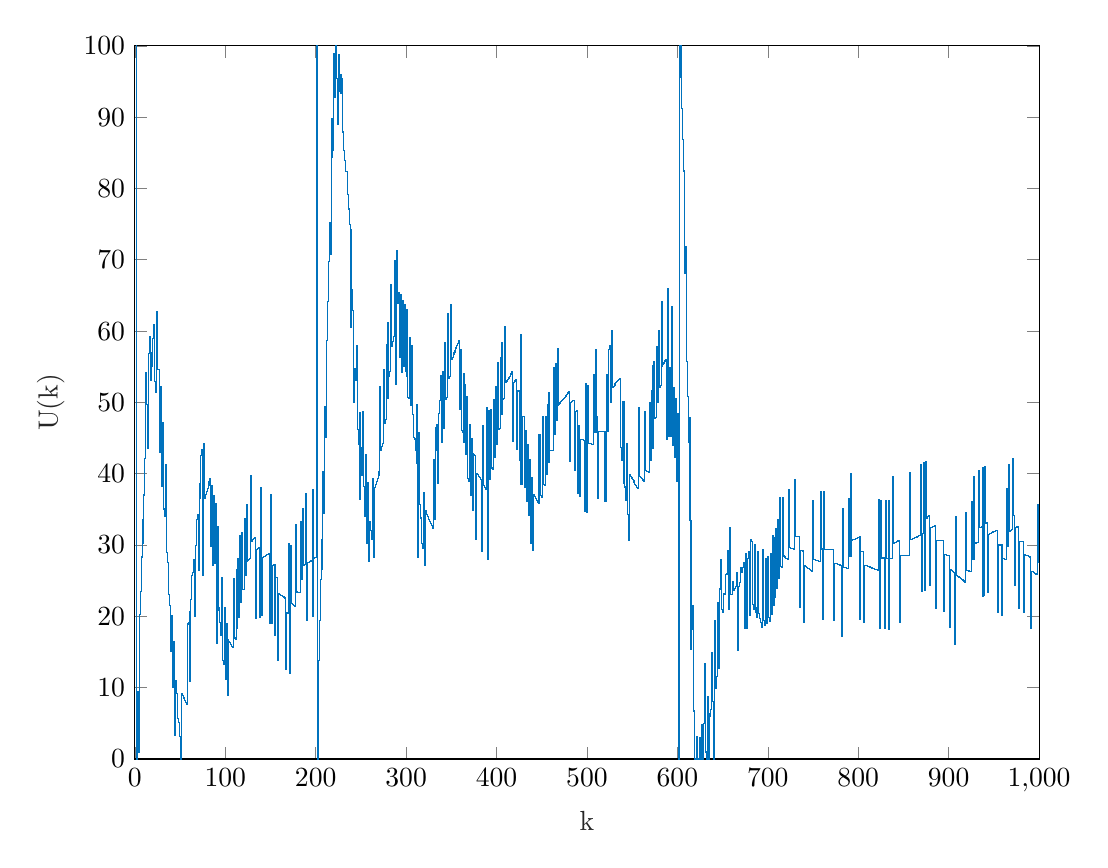
\begin{tikzpicture}

\begin{axis}[%
width=4.521in,
height=3.566in,
at={(0.758in,0.481in)},
scale only axis,
xmin=0,
xmax=1000,
xlabel style={font=\color{white!15!black}},
xlabel={k},
ymin=0,
ymax=100,
ylabel style={font=\color{white!15!black}},
ylabel={U(k)},
axis background/.style={fill=white}
]
\addplot[const plot, color=mycolor1, forget plot] table[row sep=crcr] {%
1	100\\
2	0\\
3	9.462857\\
4	0.9\\
5	20.237143\\
6	23.425714\\
7	28.32\\
8	30.27\\
9	33.621429\\
10	37.024286\\
11	42.132857\\
12	54.222857\\
13	49.74\\
14	43.482857\\
15	56.905714\\
16	59.284286\\
17	53.138571\\
18	55.092857\\
19	57.047143\\
20	59.001429\\
21	60.955714\\
22	52.984286\\
23	51.407143\\
24	62.7\\
25	54.617143\\
26	54.582857\\
27	42.917143\\
28	52.17\\
29	41.995714\\
30	38.164286\\
31	47.151429\\
32	35.057143\\
33	33.955714\\
34	41.327143\\
35	28.967143\\
36	27.6\\
37	23.125714\\
38	21.544286\\
39	16.855714\\
40	15.06\\
41	20.082857\\
42	10.024286\\
43	16.538571\\
44	3.321429\\
45	11.022857\\
46	9.222857\\
47	5.717143\\
48	5.155714\\
49	3.192857\\
50	1.178571\\
51	0\\
52	9.15\\
53	8.85\\
54	8.55\\
55	8.25\\
56	7.95\\
57	7.65\\
58	18.93\\
59	19.165714\\
60	10.877143\\
61	20.614286\\
62	22.302857\\
63	25.697143\\
64	26.147143\\
65	27.998571\\
66	19.975714\\
67	29.978571\\
68	33.587143\\
69	34.251429\\
70	26.391429\\
71	36.557143\\
72	38.674286\\
73	42.497143\\
74	43.375714\\
75	25.804286\\
76	44.232857\\
77	36.587143\\
78	37.041429\\
79	37.495714\\
80	37.95\\
81	38.404286\\
82	38.858571\\
83	39.312857\\
84	29.841429\\
85	38.344286\\
86	27.167143\\
87	36.96\\
88	27.377143\\
89	35.768571\\
90	16.208571\\
91	32.597143\\
92	21.205714\\
93	20.858571\\
94	19.11\\
95	17.31\\
96	25.384286\\
97	13.778571\\
98	13.217143\\
99	21.18\\
100	11.117143\\
101	19.028571\\
102	8.914286\\
103	16.774286\\
104	16.534286\\
105	16.294286\\
106	16.054286\\
107	15.814286\\
108	15.574286\\
109	25.26\\
110	16.971429\\
111	16.782857\\
112	26.52\\
113	18.282857\\
114	28.071429\\
115	19.885714\\
116	31.38\\
117	21.904286\\
118	31.804286\\
119	23.73\\
120	23.755714\\
121	33.707143\\
122	25.684286\\
123	35.687143\\
124	27.715714\\
125	27.844286\\
126	27.972857\\
127	28.101429\\
128	39.81\\
129	30.548571\\
130	30.737143\\
131	30.925714\\
132	31.114286\\
133	19.722857\\
134	29.301429\\
135	29.43\\
136	29.558571\\
137	29.687143\\
138	19.89\\
139	37.992857\\
140	20.095714\\
141	28.272857\\
142	28.35\\
143	28.427143\\
144	28.504286\\
145	28.581429\\
146	28.658571\\
147	28.735714\\
148	28.812857\\
149	18.964286\\
150	37.015714\\
151	19.067143\\
152	27.192857\\
153	27.218571\\
154	27.244286\\
155	17.344286\\
156	25.418571\\
157	25.392857\\
158	13.787143\\
159	23.151429\\
160	23.065714\\
161	22.98\\
162	22.894286\\
163	22.808571\\
164	22.722857\\
165	22.637143\\
166	22.551429\\
167	12.54\\
168	20.502857\\
169	20.365714\\
170	30.154286\\
171	12.042857\\
172	29.931429\\
173	21.745714\\
174	21.66\\
175	21.574286\\
176	21.488571\\
177	21.402857\\
178	32.897143\\
179	23.421429\\
180	23.395714\\
181	23.37\\
182	23.344286\\
183	33.244286\\
184	25.17\\
185	35.121429\\
186	27.098571\\
187	27.175714\\
188	27.252857\\
189	37.255714\\
190	19.358571\\
191	27.535714\\
192	27.612857\\
193	27.69\\
194	27.767143\\
195	27.844286\\
196	37.847143\\
197	19.95\\
198	28.127143\\
199	28.204286\\
200	28.281429\\
201	100\\
202	0\\
203	13.782857\\
204	19.465714\\
205	25.148571\\
206	30.831429\\
207	26.588571\\
208	40.32\\
209	34.371429\\
210	49.392857\\
211	45.038571\\
212	58.658571\\
213	64.178571\\
214	69.698571\\
215	75.218571\\
216	70.812857\\
217	84.381429\\
218	89.85\\
219	85.392857\\
220	98.91\\
221	92.747143\\
222	100\\
223	95.431429\\
224	88.985714\\
225	98.808571\\
226	93.55\\
227	93.284286\\
228	95.911429\\
229	95.431429\\
230	87.918571\\
231	85.347143\\
232	83.962857\\
233	82.415714\\
234	82.36\\
235	79.145714\\
236	77.118571\\
237	74.928571\\
238	74.23\\
239	60.447143\\
240	65.825714\\
241	62.941429\\
242	49.968571\\
243	54.807143\\
244	53.037143\\
245	58.034286\\
246	46.244286\\
247	44.045714\\
248	48.614286\\
249	36.395714\\
250	43.694286\\
251	39.785714\\
252	48.695714\\
253	38.178571\\
254	34.004286\\
255	42.648571\\
256	30.211429\\
257	38.692857\\
258	27.747143\\
259	33.07\\
260	33.237143\\
261	32.002857\\
262	30.717143\\
263	39.305714\\
264	28.214286\\
265	38.092857\\
266	38.521429\\
267	38.95\\
268	39.378571\\
269	39.807143\\
270	40.235714\\
271	52.244286\\
272	43.282857\\
273	43.771429\\
274	44.26\\
275	54.674286\\
276	47.114286\\
277	47.654286\\
278	58.12\\
279	50.611429\\
280	61.128571\\
281	53.671429\\
282	54.314286\\
283	66.537143\\
284	57.79\\
285	58.492857\\
286	59.195714\\
287	69.824286\\
288	52.552857\\
289	71.281429\\
290	63.935714\\
291	64.69\\
292	65.444286\\
293	56.272857\\
294	65.075714\\
295	54.198571\\
296	64.291429\\
297	55.008571\\
298	63.7\\
299	54.365714\\
300	63.005714\\
301	53.62\\
302	50.628571\\
303	50.581429\\
304	59.058571\\
305	49.51\\
306	57.935714\\
307	48.335714\\
308	45.13\\
309	44.868571\\
310	43.205714\\
311	41.491429\\
312	49.651429\\
313	28.205714\\
314	45.704286\\
315	35.727143\\
316	33.798571\\
317	30.164286\\
318	29.474286\\
319	37.308571\\
320	27.117143\\
321	34.9\\
322	34.582857\\
323	34.265714\\
324	33.948571\\
325	33.631429\\
326	33.314286\\
327	32.997143\\
328	32.68\\
329	32.362857\\
330	41.971429\\
331	33.605714\\
332	43.265714\\
333	46.531429\\
334	46.852857\\
335	38.65\\
336	48.472857\\
337	50.247143\\
338	53.727143\\
339	44.337143\\
340	54.322857\\
341	46.334286\\
342	56.371429\\
343	58.36\\
344	50.474286\\
345	50.688571\\
346	62.482857\\
347	53.307143\\
348	53.581429\\
349	63.781429\\
350	56.007143\\
351	56.332857\\
352	56.658571\\
353	56.984286\\
354	57.31\\
355	57.635714\\
356	57.961429\\
357	58.287143\\
358	58.612857\\
359	49.012857\\
360	57.387143\\
361	46.081429\\
362	45.82\\
363	54.082857\\
364	44.32\\
365	52.531429\\
366	42.717143\\
367	50.877143\\
368	39.357143\\
369	38.881429\\
370	46.93\\
371	36.952857\\
372	44.95\\
373	34.921429\\
374	42.867143\\
375	42.712857\\
376	42.558571\\
377	30.824286\\
378	40.06\\
379	39.845714\\
380	39.631429\\
381	39.417143\\
382	39.202857\\
383	29.062857\\
384	46.822857\\
385	38.508571\\
386	38.294286\\
387	38.08\\
388	37.865714\\
389	49.231429\\
390	28.047143\\
391	48.862857\\
392	39.258571\\
393	49.03\\
394	40.827143\\
395	40.724286\\
396	40.621429\\
397	50.444286\\
398	42.292857\\
399	52.167143\\
400	44.067143\\
401	55.647143\\
402	46.257143\\
403	46.317143\\
404	56.302857\\
405	48.314286\\
406	58.351429\\
407	50.414286\\
408	50.577143\\
409	60.665714\\
410	52.78\\
411	52.994286\\
412	53.208571\\
413	53.422857\\
414	53.637143\\
415	53.851429\\
416	54.065714\\
417	54.28\\
418	44.568571\\
419	52.831429\\
420	52.994286\\
421	53.157143\\
422	43.394286\\
423	51.605714\\
424	51.717143\\
425	41.902857\\
426	38.482857\\
427	59.512857\\
428	38.542857\\
429	47.992857\\
430	47.992857\\
431	38.067143\\
432	46.115714\\
433	36.138571\\
434	44.135714\\
435	34.107143\\
436	42.052857\\
437	41.898571\\
438	30.164286\\
439	39.4\\
440	29.26\\
441	37.094286\\
442	36.828571\\
443	36.562857\\
444	36.297143\\
445	36.031429\\
446	35.765714\\
447	45.425714\\
448	37.111429\\
449	36.897143\\
450	36.682857\\
451	48.048571\\
452	38.444286\\
453	38.29\\
454	48.061429\\
455	39.858571\\
456	49.681429\\
457	41.53\\
458	51.404286\\
459	43.304286\\
460	43.304286\\
461	43.304286\\
462	43.304286\\
463	54.884286\\
464	45.494286\\
465	55.48\\
466	47.491429\\
467	57.528571\\
468	49.591429\\
469	49.754286\\
470	49.917143\\
471	50.08\\
472	50.242857\\
473	50.405714\\
474	50.568571\\
475	50.731429\\
476	50.894286\\
477	51.057143\\
478	51.22\\
479	51.382857\\
480	51.545714\\
481	41.782857\\
482	49.994286\\
483	50.105714\\
484	50.217143\\
485	50.328571\\
486	40.514286\\
487	48.674286\\
488	48.734286\\
489	48.794286\\
490	37.274286\\
491	46.724286\\
492	36.798571\\
493	44.847143\\
494	44.795714\\
495	44.744286\\
496	44.692857\\
497	34.715714\\
498	52.638571\\
499	44.487143\\
500	34.51\\
501	52.432857\\
502	44.281429\\
503	44.23\\
504	44.178571\\
505	44.127143\\
506	44.075714\\
507	53.95\\
508	45.85\\
509	45.85\\
510	57.43\\
511	48.04\\
512	36.52\\
513	45.97\\
514	45.97\\
515	45.97\\
516	45.97\\
517	45.97\\
518	45.97\\
519	45.97\\
520	36.044286\\
521	44.092857\\
522	53.967143\\
523	45.867143\\
524	57.447143\\
525	57.982857\\
526	49.994286\\
527	60.031429\\
528	52.094286\\
529	52.257143\\
530	52.42\\
531	52.582857\\
532	52.745714\\
533	52.908571\\
534	53.071429\\
535	53.234286\\
536	53.397143\\
537	43.634286\\
538	41.92\\
539	50.08\\
540	50.14\\
541	38.62\\
542	38.144286\\
543	36.267143\\
544	44.264286\\
545	34.235714\\
546	30.601429\\
547	39.837143\\
548	39.622857\\
549	39.408571\\
550	39.194286\\
551	38.98\\
552	38.765714\\
553	38.551429\\
554	38.337143\\
555	38.122857\\
556	37.908571\\
557	49.274286\\
558	39.67\\
559	39.515714\\
560	39.361429\\
561	39.207143\\
562	39.052857\\
563	38.898571\\
564	48.67\\
565	40.467143\\
566	40.364286\\
567	40.261429\\
568	40.158571\\
569	49.981429\\
570	41.83\\
571	51.704286\\
572	43.604286\\
573	55.184286\\
574	55.72\\
575	47.731429\\
576	47.842857\\
577	57.88\\
578	49.942857\\
579	60.031429\\
580	52.145714\\
581	52.36\\
582	64.154286\\
583	54.978571\\
584	55.252857\\
585	55.527143\\
586	55.801429\\
587	56.075714\\
588	44.77\\
589	66.014286\\
590	45.258571\\
591	54.922857\\
592	45.211429\\
593	63.4\\
594	45.588571\\
595	43.925714\\
596	52.137143\\
597	42.322857\\
598	50.482857\\
599	38.962857\\
600	48.412857\\
601	0\\
602	100\\
603	100\\
604	95.611429\\
605	91.222857\\
606	86.834286\\
607	82.445714\\
608	68.131429\\
609	71.791429\\
610	55.771429\\
611	50.795714\\
612	44.418571\\
613	47.915714\\
614	33.387143\\
615	15.327143\\
616	18.185714\\
617	21.468571\\
618	6.725714\\
619	0\\
620	0\\
621	3.12\\
622	0\\
623	0\\
624	3.068571\\
625	0\\
626	0\\
627	4.894286\\
628	0\\
629	4.945714\\
630	13.422857\\
631	0.981429\\
632	0\\
633	8.691429\\
634	6.39\\
635	0\\
636	5.961429\\
637	6.93\\
638	14.931429\\
639	8.065714\\
640	0\\
641	19.422857\\
642	9.878571\\
643	11.541429\\
644	21.891429\\
645	12.724286\\
646	14.764286\\
647	23.837143\\
648	27.968571\\
649	20.987143\\
650	20.562857\\
651	23.245714\\
652	23.035714\\
653	25.932857\\
654	25.937143\\
655	29.048571\\
656	29.267143\\
657	21.012857\\
658	32.49\\
659	23.048571\\
660	23.108571\\
661	24.874286\\
662	23.695714\\
663	23.918571\\
664	24.192857\\
665	26.172857\\
666	15.282857\\
667	23.768571\\
668	24.205714\\
669	24.694286\\
670	26.888571\\
671	26.138571\\
672	26.79\\
673	27.492857\\
674	18.321429\\
675	28.83\\
676	18.368571\\
677	27.282857\\
678	28.148571\\
679	29.065714\\
680	20.108571\\
681	30.831429\\
682	30.51\\
683	21.664286\\
684	20.918571\\
685	30.098571\\
686	21.304286\\
687	20.61\\
688	19.915714\\
689	29.147143\\
690	20.404286\\
691	19.761429\\
692	19.118571\\
693	18.475714\\
694	29.412857\\
695	19.38\\
696	18.797143\\
697	28.14\\
698	19.508571\\
699	18.977143\\
700	28.371429\\
701	19.791429\\
702	19.311429\\
703	28.757143\\
704	20.228571\\
705	31.38\\
706	21.561429\\
707	31.118571\\
708	22.701429\\
709	32.31\\
710	23.944286\\
711	33.604286\\
712	25.29\\
713	36.655714\\
714	27.051429\\
715	26.897143\\
716	36.668571\\
717	28.465714\\
718	28.362857\\
719	28.26\\
720	28.157143\\
721	28.054286\\
722	27.951429\\
723	37.774286\\
724	29.622857\\
725	29.571429\\
726	29.52\\
727	29.468571\\
728	29.417143\\
729	29.365714\\
730	39.24\\
731	31.14\\
732	31.14\\
733	31.14\\
734	31.14\\
735	21.214286\\
736	29.262857\\
737	29.211429\\
738	29.16\\
739	19.182857\\
740	27.18\\
741	27.077143\\
742	26.974286\\
743	26.871429\\
744	26.768571\\
745	26.665714\\
746	26.562857\\
747	26.46\\
748	26.357143\\
749	36.18\\
750	28.028571\\
751	27.977143\\
752	27.925714\\
753	27.874286\\
754	27.822857\\
755	27.771429\\
756	27.72\\
757	27.668571\\
758	37.542857\\
759	29.442857\\
760	19.517143\\
761	27.565714\\
762	37.44\\
763	29.34\\
764	29.34\\
765	29.34\\
766	29.34\\
767	29.34\\
768	29.34\\
769	29.34\\
770	29.34\\
771	29.34\\
772	29.34\\
773	19.414286\\
774	27.462857\\
775	27.411429\\
776	27.36\\
777	27.308571\\
778	27.257143\\
779	27.205714\\
780	27.154286\\
781	27.102857\\
782	17.125714\\
783	35.048571\\
784	26.897143\\
785	26.845714\\
786	26.794286\\
787	26.742857\\
788	26.691429\\
789	36.565714\\
790	28.465714\\
791	28.465714\\
792	40.045714\\
793	30.655714\\
794	30.715714\\
795	30.775714\\
796	30.835714\\
797	30.895714\\
798	30.955714\\
799	31.015714\\
800	31.075714\\
801	31.135714\\
802	19.615714\\
803	29.065714\\
804	29.065714\\
805	29.065714\\
806	19.14\\
807	27.188571\\
808	27.137143\\
809	27.085714\\
810	27.034286\\
811	26.982857\\
812	26.931429\\
813	26.88\\
814	26.828571\\
815	26.777143\\
816	26.725714\\
817	26.674286\\
818	26.622857\\
819	26.571429\\
820	26.52\\
821	26.468571\\
822	36.342857\\
823	28.242857\\
824	18.317143\\
825	36.291429\\
826	28.191429\\
827	28.191429\\
828	28.191429\\
829	18.265714\\
830	36.24\\
831	28.14\\
832	28.14\\
833	18.214286\\
834	36.188571\\
835	28.088571\\
836	28.088571\\
837	28.088571\\
838	39.668571\\
839	30.278571\\
840	30.338571\\
841	30.398571\\
842	30.458571\\
843	30.518571\\
844	30.578571\\
845	30.638571\\
846	19.118571\\
847	28.568571\\
848	28.568571\\
849	28.568571\\
850	28.568571\\
851	28.568571\\
852	28.568571\\
853	28.568571\\
854	28.568571\\
855	28.568571\\
856	28.568571\\
857	40.148571\\
858	30.758571\\
859	30.818571\\
860	30.878571\\
861	30.938571\\
862	30.998571\\
863	31.058571\\
864	31.118571\\
865	31.178571\\
866	31.238571\\
867	31.298571\\
868	31.358571\\
869	41.344286\\
870	23.43\\
871	31.59\\
872	41.575714\\
873	23.661429\\
874	41.747143\\
875	33.758571\\
876	33.87\\
877	33.981429\\
878	34.092857\\
879	24.278571\\
880	32.438571\\
881	32.498571\\
882	32.558571\\
883	32.618571\\
884	32.678571\\
885	21.158571\\
886	30.608571\\
887	30.608571\\
888	30.608571\\
889	30.608571\\
890	30.608571\\
891	30.608571\\
892	30.608571\\
893	30.608571\\
894	20.682857\\
895	28.731429\\
896	28.68\\
897	28.628571\\
898	28.577143\\
899	28.525714\\
900	28.474286\\
901	18.497143\\
902	26.494286\\
903	26.391429\\
904	26.288571\\
905	26.185714\\
906	26.082857\\
907	16.054286\\
908	33.925714\\
909	25.722857\\
910	25.62\\
911	25.517143\\
912	25.414286\\
913	25.311429\\
914	25.208571\\
915	25.105714\\
916	25.002857\\
917	24.9\\
918	24.797143\\
919	34.62\\
920	26.468571\\
921	26.417143\\
922	26.365714\\
923	26.314286\\
924	26.262857\\
925	36.137143\\
926	28.037143\\
927	28.037143\\
928	39.617143\\
929	30.227143\\
930	30.287143\\
931	30.347143\\
932	30.407143\\
933	40.392857\\
934	32.404286\\
935	32.515714\\
936	32.627143\\
937	22.812857\\
938	40.898571\\
939	22.984286\\
940	41.07\\
941	33.081429\\
942	33.192857\\
943	23.378571\\
944	31.538571\\
945	31.598571\\
946	31.658571\\
947	31.718571\\
948	31.778571\\
949	31.838571\\
950	31.898571\\
951	31.958571\\
952	32.018571\\
953	32.078571\\
954	20.558571\\
955	30.008571\\
956	30.008571\\
957	30.008571\\
958	30.008571\\
959	20.082857\\
960	28.131429\\
961	28.08\\
962	28.028571\\
963	27.977143\\
964	37.851429\\
965	29.751429\\
966	41.331429\\
967	31.941429\\
968	32.001429\\
969	32.061429\\
970	32.121429\\
971	42.107143\\
972	34.118571\\
973	24.304286\\
974	32.464286\\
975	32.524286\\
976	32.584286\\
977	21.064286\\
978	30.514286\\
979	30.514286\\
980	30.514286\\
981	30.514286\\
982	30.514286\\
983	20.588571\\
984	28.637143\\
985	28.585714\\
986	28.534286\\
987	28.482857\\
988	28.431429\\
989	28.38\\
990	28.328571\\
991	18.351429\\
992	26.348571\\
993	26.245714\\
994	26.142857\\
995	26.04\\
996	25.937143\\
997	25.834286\\
998	35.657143\\
999	27.505714\\
1000	27.454286\\
};
\end{axis}
\end{tikzpicture}%
\caption{Sterowanie procesu z regulatorem PID dla parametrów $K = 30$,  $T_i = 35$,  $T_d = 4.5$}
\end{figure}

Wskaźnik jakości regulacji dla PID:

\begin{equation}
E = 3,043e+3
\end{equation}

\begin{figure}[H]
\centering
% This file was created by matlab2tikz.
%
%The latest updates can be retrieved from
%  http://www.mathworks.com/matlabcentral/fileexchange/22022-matlab2tikz-matlab2tikz
%where you can also make suggestions and rate matlab2tikz.
%
\definecolor{mycolor1}{rgb}{0.00000,0.44700,0.74100}%
%
\begin{tikzpicture}

\begin{axis}[%
width=4.521in,
height=3.566in,
at={(0.758in,0.481in)},
scale only axis,
xmin=0,
xmax=1000,
xlabel style={font=\color{white!15!black}},
xlabel={k},
ymin=26,
ymax=36,
ylabel style={font=\color{white!15!black}},
ylabel={Y(k)},
axis background/.style={fill=white}
]
\addplot[const plot, color=mycolor1, forget plot] table[row sep=crcr] {%
1	28.37\\
2	28.37\\
3	28.31\\
4	28.31\\
5	28.25\\
6	28.06\\
7	27.93\\
8	27.81\\
9	27.68\\
10	27.5\\
11	27.37\\
12	27.25\\
13	27.12\\
14	27\\
15	26.93\\
16	26.87\\
17	26.81\\
18	26.75\\
19	26.75\\
20	26.68\\
21	26.68\\
22	26.68\\
23	26.68\\
24	26.62\\
25	26.62\\
26	26.68\\
27	26.68\\
28	26.75\\
29	26.75\\
30	26.81\\
31	26.87\\
32	26.87\\
33	26.93\\
34	27\\
35	27.06\\
36	27.12\\
37	27.18\\
38	27.25\\
39	27.37\\
40	27.43\\
41	27.5\\
42	27.56\\
43	27.62\\
44	27.68\\
45	27.75\\
46	27.81\\
47	27.87\\
48	27.93\\
49	28\\
50	28.06\\
51	28.12\\
52	28.18\\
53	28.25\\
54	28.31\\
55	28.37\\
56	28.37\\
57	28.43\\
58	28.5\\
59	28.5\\
60	28.56\\
61	28.56\\
62	28.62\\
63	28.62\\
64	28.62\\
65	28.62\\
66	28.62\\
67	28.62\\
68	28.62\\
69	28.62\\
70	28.62\\
71	28.62\\
72	28.56\\
73	28.56\\
74	28.56\\
75	28.56\\
76	28.56\\
77	28.56\\
78	28.56\\
79	28.56\\
80	28.56\\
81	28.56\\
82	28.62\\
83	28.62\\
84	28.62\\
85	28.62\\
86	28.62\\
87	28.62\\
88	28.62\\
89	28.62\\
90	28.62\\
91	28.68\\
92	28.68\\
93	28.62\\
94	28.68\\
95	28.68\\
96	28.68\\
97	28.75\\
98	28.75\\
99	28.75\\
100	28.75\\
101	28.75\\
102	28.75\\
103	28.75\\
104	28.75\\
105	28.81\\
106	28.87\\
107	28.81\\
108	28.87\\
109	28.87\\
110	28.87\\
111	28.87\\
112	28.87\\
113	28.93\\
114	28.93\\
115	28.93\\
116	28.93\\
117	28.93\\
118	28.93\\
119	28.93\\
120	28.93\\
121	28.93\\
122	28.93\\
123	28.93\\
124	28.93\\
125	28.93\\
126	28.93\\
127	28.93\\
128	28.93\\
129	28.93\\
130	28.93\\
131	28.87\\
132	28.87\\
133	28.87\\
134	28.87\\
135	28.81\\
136	28.81\\
137	28.81\\
138	28.75\\
139	28.75\\
140	28.75\\
141	28.75\\
142	28.75\\
143	28.75\\
144	28.75\\
145	28.75\\
146	28.68\\
147	28.68\\
148	28.68\\
149	28.68\\
150	28.68\\
151	28.68\\
152	28.68\\
153	28.68\\
154	28.68\\
155	28.68\\
156	28.68\\
157	28.68\\
158	28.75\\
159	28.75\\
160	28.75\\
161	28.75\\
162	28.75\\
163	28.75\\
164	28.75\\
165	28.81\\
166	28.75\\
167	28.75\\
168	28.75\\
169	28.75\\
170	28.75\\
171	28.75\\
172	28.81\\
173	28.81\\
174	28.81\\
175	28.81\\
176	28.87\\
177	28.87\\
178	28.87\\
179	28.87\\
180	28.93\\
181	28.93\\
182	28.93\\
183	28.93\\
184	28.93\\
185	28.93\\
186	28.93\\
187	28.87\\
188	28.93\\
189	28.93\\
190	28.87\\
191	28.87\\
192	28.87\\
193	28.87\\
194	28.87\\
195	28.87\\
196	28.81\\
197	28.81\\
198	28.81\\
199	28.75\\
200	28.81\\
201	28.75\\
202	28.75\\
203	28.75\\
204	28.75\\
205	28.75\\
206	28.75\\
207	28.68\\
208	28.75\\
209	28.68\\
210	28.75\\
211	28.75\\
212	28.81\\
213	28.81\\
214	28.87\\
215	28.93\\
216	29\\
217	29.06\\
218	29.18\\
219	29.25\\
220	29.37\\
221	29.5\\
222	29.62\\
223	29.75\\
224	29.93\\
225	30.06\\
226	30.18\\
227	30.37\\
228	30.5\\
229	30.68\\
230	30.87\\
231	31\\
232	31.12\\
233	31.31\\
234	31.43\\
235	31.56\\
236	31.68\\
237	31.87\\
238	32\\
239	32.12\\
240	32.25\\
241	32.31\\
242	32.43\\
243	32.5\\
244	32.62\\
245	32.68\\
246	32.75\\
247	32.81\\
248	32.87\\
249	32.93\\
250	33\\
251	33.06\\
252	33.06\\
253	33.06\\
254	33.06\\
255	33.12\\
256	33.12\\
257	33.06\\
258	33.06\\
259	33.06\\
260	33.06\\
261	33.06\\
262	33.06\\
263	33.06\\
264	33\\
265	33\\
266	33\\
267	33\\
268	33\\
269	33\\
270	33\\
271	33\\
272	33\\
273	33\\
274	33\\
275	33\\
276	33\\
277	33.06\\
278	33.06\\
279	33.12\\
280	33.12\\
281	33.18\\
282	33.18\\
283	33.25\\
284	33.25\\
285	33.31\\
286	33.37\\
287	33.37\\
288	33.43\\
289	33.5\\
290	33.5\\
291	33.56\\
292	33.62\\
293	33.68\\
294	33.75\\
295	33.81\\
296	33.87\\
297	33.87\\
298	33.93\\
299	33.93\\
300	34\\
301	34.06\\
302	34.12\\
303	34.12\\
304	34.18\\
305	34.18\\
306	34.18\\
307	34.18\\
308	34.18\\
309	34.18\\
310	34.12\\
311	34.12\\
312	34.12\\
313	34.12\\
314	34.12\\
315	34.06\\
316	34.06\\
317	34\\
318	34\\
319	34\\
320	33.93\\
321	33.93\\
322	33.87\\
323	33.87\\
324	33.87\\
325	33.87\\
326	33.81\\
327	33.81\\
328	33.81\\
329	33.81\\
330	33.81\\
331	33.81\\
332	33.81\\
333	33.81\\
334	33.81\\
335	33.87\\
336	33.87\\
337	33.93\\
338	34\\
339	34\\
340	34.06\\
341	34.06\\
342	34.12\\
343	34.18\\
344	34.18\\
345	34.18\\
346	34.25\\
347	34.25\\
348	34.31\\
349	34.37\\
350	34.43\\
351	34.43\\
352	34.5\\
353	34.5\\
354	34.56\\
355	34.62\\
356	34.62\\
357	34.62\\
358	34.68\\
359	34.75\\
360	34.75\\
361	34.81\\
362	34.81\\
363	34.87\\
364	34.87\\
365	34.87\\
366	34.93\\
367	34.93\\
368	35\\
369	35\\
370	35\\
371	35\\
372	35\\
373	35\\
374	35\\
375	34.93\\
376	34.93\\
377	34.93\\
378	34.93\\
379	34.93\\
380	34.87\\
381	34.87\\
382	34.87\\
383	34.81\\
384	34.81\\
385	34.81\\
386	34.81\\
387	34.81\\
388	34.81\\
389	34.81\\
390	34.75\\
391	34.75\\
392	34.75\\
393	34.75\\
394	34.75\\
395	34.75\\
396	34.75\\
397	34.75\\
398	34.75\\
399	34.75\\
400	34.81\\
401	34.81\\
402	34.81\\
403	34.81\\
404	34.87\\
405	34.87\\
406	34.87\\
407	34.87\\
408	34.87\\
409	34.87\\
410	34.87\\
411	34.93\\
412	34.93\\
413	34.93\\
414	34.93\\
415	35\\
416	35\\
417	35.06\\
418	35.12\\
419	35.12\\
420	35.12\\
421	35.18\\
422	35.18\\
423	35.18\\
424	35.18\\
425	35.18\\
426	35.18\\
427	35.18\\
428	35.18\\
429	35.12\\
430	35.12\\
431	35.06\\
432	35.06\\
433	35\\
434	35\\
435	34.93\\
436	34.93\\
437	34.93\\
438	34.93\\
439	34.93\\
440	34.93\\
441	35\\
442	35\\
443	35.06\\
444	35.12\\
445	35.12\\
446	35.12\\
447	35.12\\
448	35.18\\
449	35.18\\
450	35.18\\
451	35.25\\
452	35.25\\
453	35.31\\
454	35.31\\
455	35.31\\
456	35.37\\
457	35.37\\
458	35.43\\
459	35.5\\
460	35.5\\
461	35.5\\
462	35.56\\
463	35.62\\
464	35.62\\
465	35.62\\
466	35.62\\
467	35.68\\
468	35.68\\
469	35.68\\
470	35.62\\
471	35.62\\
472	35.62\\
473	35.62\\
474	35.62\\
475	35.56\\
476	35.5\\
477	35.5\\
478	35.43\\
479	35.43\\
480	35.37\\
481	35.37\\
482	35.37\\
483	35.37\\
484	35.37\\
485	35.37\\
486	35.37\\
487	35.37\\
488	35.37\\
489	35.37\\
490	35.37\\
491	35.37\\
492	35.31\\
493	35.31\\
494	35.31\\
495	35.31\\
496	35.31\\
497	35.31\\
498	35.25\\
499	35.25\\
500	35.25\\
501	35.25\\
502	35.31\\
503	35.31\\
504	35.25\\
505	35.25\\
506	35.25\\
507	35.18\\
508	35.18\\
509	35.18\\
510	35.18\\
511	35.18\\
512	35.18\\
513	35.18\\
514	35.18\\
515	35.18\\
516	35.18\\
517	35.18\\
518	35.18\\
519	35.25\\
520	35.25\\
521	35.25\\
522	35.25\\
523	35.25\\
524	35.25\\
525	35.25\\
526	35.25\\
527	35.25\\
528	35.25\\
529	35.25\\
530	35.18\\
531	35.25\\
532	35.18\\
533	35.18\\
534	35.18\\
535	35.18\\
536	35.18\\
537	35.18\\
538	35.18\\
539	35.18\\
540	35.18\\
541	35.18\\
542	35.18\\
543	35.18\\
544	35.18\\
545	35.25\\
546	35.18\\
547	35.25\\
548	35.25\\
549	35.25\\
550	35.25\\
551	35.25\\
552	35.25\\
553	35.25\\
554	35.31\\
555	35.25\\
556	35.25\\
557	35.25\\
558	35.25\\
559	35.25\\
560	35.25\\
561	35.18\\
562	35.18\\
563	35.18\\
564	35.18\\
565	35.18\\
566	35.25\\
567	35.25\\
568	35.25\\
569	35.31\\
570	35.31\\
571	35.37\\
572	35.37\\
573	35.37\\
574	35.37\\
575	35.31\\
576	35.31\\
577	35.25\\
578	35.25\\
579	35.25\\
580	35.18\\
581	35.18\\
582	35.18\\
583	35.18\\
584	35.18\\
585	35.18\\
586	35.18\\
587	35.18\\
588	35.18\\
589	35.18\\
590	35.18\\
591	35.25\\
592	35.25\\
593	35.25\\
594	35.25\\
595	35.25\\
596	35.31\\
597	35.31\\
598	35.31\\
599	35.31\\
600	35.31\\
601	35.31\\
602	35.37\\
603	35.31\\
604	35.31\\
605	35.31\\
606	35.25\\
607	35.25\\
608	35.25\\
609	35.18\\
610	35.18\\
611	35.12\\
612	35.12\\
613	35.06\\
614	35\\
615	34.93\\
616	34.87\\
617	34.81\\
618	34.75\\
619	34.62\\
620	34.56\\
621	34.43\\
622	34.31\\
623	34.18\\
624	34.06\\
625	33.93\\
626	33.81\\
627	33.68\\
628	33.56\\
629	33.43\\
630	33.31\\
631	33.18\\
632	33.06\\
633	32.93\\
634	32.81\\
635	32.75\\
636	32.62\\
637	32.5\\
638	32.37\\
639	32.31\\
640	32.25\\
641	32.18\\
642	32.12\\
643	32.12\\
644	32.06\\
645	32.06\\
646	32\\
647	32\\
648	31.93\\
649	31.93\\
650	31.87\\
651	31.87\\
652	31.81\\
653	31.81\\
654	31.75\\
655	31.81\\
656	31.75\\
657	31.75\\
658	31.75\\
659	31.75\\
660	31.75\\
661	31.75\\
662	31.75\\
663	31.81\\
664	31.81\\
665	31.87\\
666	31.87\\
667	31.87\\
668	31.93\\
669	31.87\\
670	31.93\\
671	31.93\\
672	31.93\\
673	31.93\\
674	31.87\\
675	31.87\\
676	31.87\\
677	31.87\\
678	31.81\\
679	31.81\\
680	31.75\\
681	31.75\\
682	31.68\\
683	31.62\\
684	31.56\\
685	31.5\\
686	31.43\\
687	31.43\\
688	31.37\\
689	31.31\\
690	31.18\\
691	31.18\\
692	31.12\\
693	31.06\\
694	31\\
695	30.93\\
696	30.93\\
697	30.87\\
698	30.81\\
699	30.81\\
700	30.81\\
701	30.75\\
702	30.75\\
703	30.75\\
704	30.75\\
705	30.75\\
706	30.75\\
707	30.75\\
708	30.75\\
709	30.75\\
710	30.75\\
711	30.75\\
712	30.75\\
713	30.75\\
714	30.75\\
715	30.75\\
716	30.75\\
717	30.75\\
718	30.75\\
719	30.75\\
720	30.75\\
721	30.81\\
722	30.81\\
723	30.81\\
724	30.75\\
725	30.75\\
726	30.81\\
727	30.81\\
728	30.81\\
729	30.75\\
730	30.81\\
731	30.81\\
732	30.81\\
733	30.81\\
734	30.81\\
735	30.81\\
736	30.81\\
737	30.81\\
738	30.81\\
739	30.75\\
740	30.75\\
741	30.75\\
742	30.68\\
743	30.68\\
744	30.68\\
745	30.62\\
746	30.62\\
747	30.56\\
748	30.56\\
749	30.5\\
750	30.5\\
751	30.5\\
752	30.43\\
753	30.5\\
754	30.43\\
755	30.43\\
756	30.43\\
757	30.37\\
758	30.37\\
759	30.37\\
760	30.31\\
761	30.31\\
762	30.31\\
763	30.25\\
764	30.25\\
765	30.25\\
766	30.18\\
767	30.18\\
768	30.18\\
769	30.18\\
770	30.18\\
771	30.18\\
772	30.18\\
773	30.18\\
774	30.18\\
775	30.18\\
776	30.18\\
777	30.18\\
778	30.18\\
779	30.18\\
780	30.18\\
781	30.18\\
782	30.18\\
783	30.18\\
784	30.18\\
785	30.18\\
786	30.18\\
787	30.12\\
788	30.18\\
789	30.18\\
790	30.12\\
791	30.18\\
792	30.18\\
793	30.18\\
794	30.18\\
795	30.25\\
796	30.25\\
797	30.18\\
798	30.25\\
799	30.18\\
800	30.18\\
801	30.18\\
802	30.18\\
803	30.18\\
804	30.12\\
805	30.12\\
806	30.12\\
807	30.12\\
808	30.12\\
809	30.12\\
810	30.12\\
811	30.12\\
812	30.12\\
813	30.12\\
814	30.12\\
815	30.12\\
816	30.12\\
817	30.12\\
818	30.12\\
819	30.06\\
820	30.06\\
821	30.06\\
822	30.06\\
823	30.06\\
824	30\\
825	30.06\\
826	30.06\\
827	30\\
828	30\\
829	30.06\\
830	30\\
831	30\\
832	30\\
833	30\\
834	30\\
835	30\\
836	30\\
837	30.06\\
838	30.06\\
839	30\\
840	30.06\\
841	30\\
842	30.06\\
843	30\\
844	30\\
845	30\\
846	30\\
847	30\\
848	30\\
849	30\\
850	30\\
851	29.93\\
852	30\\
853	29.93\\
854	29.93\\
855	29.93\\
856	29.87\\
857	29.87\\
858	29.87\\
859	29.87\\
860	29.87\\
861	29.81\\
862	29.81\\
863	29.81\\
864	29.81\\
865	29.81\\
866	29.81\\
867	29.81\\
868	29.81\\
869	29.81\\
870	29.81\\
871	29.81\\
872	29.87\\
873	29.81\\
874	29.81\\
875	29.81\\
876	29.75\\
877	29.81\\
878	29.75\\
879	29.75\\
880	29.75\\
881	29.68\\
882	29.68\\
883	29.68\\
884	29.68\\
885	29.68\\
886	29.62\\
887	29.68\\
888	29.68\\
889	29.68\\
890	29.68\\
891	29.68\\
892	29.68\\
893	29.68\\
894	29.68\\
895	29.68\\
896	29.68\\
897	29.68\\
898	29.62\\
899	29.62\\
900	29.62\\
901	29.62\\
902	29.56\\
903	29.56\\
904	29.62\\
905	29.62\\
906	29.62\\
907	29.62\\
908	29.68\\
909	29.68\\
910	29.68\\
911	29.75\\
912	29.75\\
913	29.75\\
914	29.81\\
915	29.81\\
916	29.81\\
917	29.87\\
918	29.87\\
919	29.87\\
920	29.87\\
921	29.87\\
922	29.87\\
923	29.81\\
924	29.81\\
925	29.81\\
926	29.81\\
927	29.81\\
928	29.81\\
929	29.81\\
930	29.75\\
931	29.75\\
932	29.75\\
933	29.75\\
934	29.81\\
935	29.75\\
936	29.75\\
937	29.81\\
938	29.81\\
939	29.87\\
940	29.81\\
941	29.87\\
942	29.87\\
943	29.87\\
944	29.87\\
945	29.93\\
946	29.93\\
947	29.93\\
948	30\\
949	30\\
950	30\\
951	30\\
952	30\\
953	30\\
954	30\\
955	30\\
956	30\\
957	30\\
958	30\\
959	30\\
960	30\\
961	30\\
962	30\\
963	30\\
964	30\\
965	30\\
966	30\\
967	30\\
968	30\\
969	30\\
970	30\\
971	30\\
972	30\\
973	30\\
974	30\\
975	30\\
976	29.93\\
977	29.93\\
978	29.93\\
979	29.87\\
980	29.87\\
981	29.87\\
982	29.81\\
983	29.81\\
984	29.87\\
985	29.81\\
986	29.81\\
987	29.81\\
988	29.81\\
989	29.81\\
990	29.81\\
991	29.81\\
992	29.81\\
993	29.81\\
994	29.81\\
995	29.81\\
996	29.81\\
997	29.81\\
998	29.87\\
999	29.87\\
1000	29.87\\
};
\addplot [color=red, dashed, forget plot]
  table[row sep=crcr]{%
1	28.4\\
2	28.4\\
3	28.4\\
4	28.4\\
5	28.4\\
6	28.4\\
7	28.4\\
8	28.4\\
9	28.4\\
10	28.4\\
11	28.4\\
12	28.4\\
13	28.4\\
14	28.4\\
15	28.4\\
16	28.4\\
17	28.4\\
18	28.4\\
19	28.4\\
20	28.4\\
21	28.4\\
22	28.4\\
23	28.4\\
24	28.4\\
25	28.4\\
26	28.4\\
27	28.4\\
28	28.4\\
29	28.4\\
30	28.4\\
31	28.4\\
32	28.4\\
33	28.4\\
34	28.4\\
35	28.4\\
36	28.4\\
37	28.4\\
38	28.4\\
39	28.4\\
40	28.4\\
41	28.4\\
42	28.4\\
43	28.4\\
44	28.4\\
45	28.4\\
46	28.4\\
47	28.4\\
48	28.4\\
49	28.4\\
50	28.4\\
51	28.4\\
52	28.4\\
53	28.4\\
54	28.4\\
55	28.4\\
56	28.4\\
57	28.4\\
58	28.4\\
59	28.4\\
60	28.4\\
61	28.4\\
62	28.4\\
63	28.4\\
64	28.4\\
65	28.4\\
66	28.4\\
67	28.4\\
68	28.4\\
69	28.4\\
70	28.4\\
71	28.4\\
72	28.4\\
73	28.4\\
74	28.4\\
75	28.4\\
76	28.4\\
77	28.4\\
78	28.4\\
79	28.4\\
80	28.4\\
81	28.4\\
82	28.4\\
83	28.4\\
84	28.4\\
85	28.4\\
86	28.4\\
87	28.4\\
88	28.4\\
89	28.4\\
90	28.4\\
91	28.4\\
92	28.4\\
93	28.4\\
94	28.4\\
95	28.4\\
96	28.4\\
97	28.4\\
98	28.4\\
99	28.4\\
100	28.4\\
101	28.4\\
102	28.4\\
103	28.4\\
104	28.4\\
105	28.4\\
106	28.4\\
107	28.4\\
108	28.4\\
109	28.4\\
110	28.4\\
111	28.4\\
112	28.4\\
113	28.4\\
114	28.4\\
115	28.4\\
116	28.4\\
117	28.4\\
118	28.4\\
119	28.4\\
120	28.4\\
121	28.4\\
122	28.4\\
123	28.4\\
124	28.4\\
125	28.4\\
126	28.4\\
127	28.4\\
128	28.4\\
129	28.4\\
130	28.4\\
131	28.4\\
132	28.4\\
133	28.4\\
134	28.4\\
135	28.4\\
136	28.4\\
137	28.4\\
138	28.4\\
139	28.4\\
140	28.4\\
141	28.4\\
142	28.4\\
143	28.4\\
144	28.4\\
145	28.4\\
146	28.4\\
147	28.4\\
148	28.4\\
149	28.4\\
150	28.4\\
151	28.4\\
152	28.4\\
153	28.4\\
154	28.4\\
155	28.4\\
156	28.4\\
157	28.4\\
158	28.4\\
159	28.4\\
160	28.4\\
161	28.4\\
162	28.4\\
163	28.4\\
164	28.4\\
165	28.4\\
166	28.4\\
167	28.4\\
168	28.4\\
169	28.4\\
170	28.4\\
171	28.4\\
172	28.4\\
173	28.4\\
174	28.4\\
175	28.4\\
176	28.4\\
177	28.4\\
178	28.4\\
179	28.4\\
180	28.4\\
181	28.4\\
182	28.4\\
183	28.4\\
184	28.4\\
185	28.4\\
186	28.4\\
187	28.4\\
188	28.4\\
189	28.4\\
190	28.4\\
191	28.4\\
192	28.4\\
193	28.4\\
194	28.4\\
195	28.4\\
196	28.4\\
197	28.4\\
198	28.4\\
199	28.4\\
200	28.4\\
201	35\\
202	35\\
203	35\\
204	35\\
205	35\\
206	35\\
207	35\\
208	35\\
209	35\\
210	35\\
211	35\\
212	35\\
213	35\\
214	35\\
215	35\\
216	35\\
217	35\\
218	35\\
219	35\\
220	35\\
221	35\\
222	35\\
223	35\\
224	35\\
225	35\\
226	35\\
227	35\\
228	35\\
229	35\\
230	35\\
231	35\\
232	35\\
233	35\\
234	35\\
235	35\\
236	35\\
237	35\\
238	35\\
239	35\\
240	35\\
241	35\\
242	35\\
243	35\\
244	35\\
245	35\\
246	35\\
247	35\\
248	35\\
249	35\\
250	35\\
251	35\\
252	35\\
253	35\\
254	35\\
255	35\\
256	35\\
257	35\\
258	35\\
259	35\\
260	35\\
261	35\\
262	35\\
263	35\\
264	35\\
265	35\\
266	35\\
267	35\\
268	35\\
269	35\\
270	35\\
271	35\\
272	35\\
273	35\\
274	35\\
275	35\\
276	35\\
277	35\\
278	35\\
279	35\\
280	35\\
281	35\\
282	35\\
283	35\\
284	35\\
285	35\\
286	35\\
287	35\\
288	35\\
289	35\\
290	35\\
291	35\\
292	35\\
293	35\\
294	35\\
295	35\\
296	35\\
297	35\\
298	35\\
299	35\\
300	35\\
301	35\\
302	35\\
303	35\\
304	35\\
305	35\\
306	35\\
307	35\\
308	35\\
309	35\\
310	35\\
311	35\\
312	35\\
313	35\\
314	35\\
315	35\\
316	35\\
317	35\\
318	35\\
319	35\\
320	35\\
321	35\\
322	35\\
323	35\\
324	35\\
325	35\\
326	35\\
327	35\\
328	35\\
329	35\\
330	35\\
331	35\\
332	35\\
333	35\\
334	35\\
335	35\\
336	35\\
337	35\\
338	35\\
339	35\\
340	35\\
341	35\\
342	35\\
343	35\\
344	35\\
345	35\\
346	35\\
347	35\\
348	35\\
349	35\\
350	35\\
351	35\\
352	35\\
353	35\\
354	35\\
355	35\\
356	35\\
357	35\\
358	35\\
359	35\\
360	35\\
361	35\\
362	35\\
363	35\\
364	35\\
365	35\\
366	35\\
367	35\\
368	35\\
369	35\\
370	35\\
371	35\\
372	35\\
373	35\\
374	35\\
375	35\\
376	35\\
377	35\\
378	35\\
379	35\\
380	35\\
381	35\\
382	35\\
383	35\\
384	35\\
385	35\\
386	35\\
387	35\\
388	35\\
389	35\\
390	35\\
391	35\\
392	35\\
393	35\\
394	35\\
395	35\\
396	35\\
397	35\\
398	35\\
399	35\\
400	35\\
401	35\\
402	35\\
403	35\\
404	35\\
405	35\\
406	35\\
407	35\\
408	35\\
409	35\\
410	35\\
411	35\\
412	35\\
413	35\\
414	35\\
415	35\\
416	35\\
417	35\\
418	35\\
419	35\\
420	35\\
421	35\\
422	35\\
423	35\\
424	35\\
425	35\\
426	35\\
427	35\\
428	35\\
429	35\\
430	35\\
431	35\\
432	35\\
433	35\\
434	35\\
435	35\\
436	35\\
437	35\\
438	35\\
439	35\\
440	35\\
441	35\\
442	35\\
443	35\\
444	35\\
445	35\\
446	35\\
447	35\\
448	35\\
449	35\\
450	35\\
451	35\\
452	35\\
453	35\\
454	35\\
455	35\\
456	35\\
457	35\\
458	35\\
459	35\\
460	35\\
461	35\\
462	35\\
463	35\\
464	35\\
465	35\\
466	35\\
467	35\\
468	35\\
469	35\\
470	35\\
471	35\\
472	35\\
473	35\\
474	35\\
475	35\\
476	35\\
477	35\\
478	35\\
479	35\\
480	35\\
481	35\\
482	35\\
483	35\\
484	35\\
485	35\\
486	35\\
487	35\\
488	35\\
489	35\\
490	35\\
491	35\\
492	35\\
493	35\\
494	35\\
495	35\\
496	35\\
497	35\\
498	35\\
499	35\\
500	35\\
501	35\\
502	35\\
503	35\\
504	35\\
505	35\\
506	35\\
507	35\\
508	35\\
509	35\\
510	35\\
511	35\\
512	35\\
513	35\\
514	35\\
515	35\\
516	35\\
517	35\\
518	35\\
519	35\\
520	35\\
521	35\\
522	35\\
523	35\\
524	35\\
525	35\\
526	35\\
527	35\\
528	35\\
529	35\\
530	35\\
531	35\\
532	35\\
533	35\\
534	35\\
535	35\\
536	35\\
537	35\\
538	35\\
539	35\\
540	35\\
541	35\\
542	35\\
543	35\\
544	35\\
545	35\\
546	35\\
547	35\\
548	35\\
549	35\\
550	35\\
551	35\\
552	35\\
553	35\\
554	35\\
555	35\\
556	35\\
557	35\\
558	35\\
559	35\\
560	35\\
561	35\\
562	35\\
563	35\\
564	35\\
565	35\\
566	35\\
567	35\\
568	35\\
569	35\\
570	35\\
571	35\\
572	35\\
573	35\\
574	35\\
575	35\\
576	35\\
577	35\\
578	35\\
579	35\\
580	35\\
581	35\\
582	35\\
583	35\\
584	35\\
585	35\\
586	35\\
587	35\\
588	35\\
589	35\\
590	35\\
591	35\\
592	35\\
593	35\\
594	35\\
595	35\\
596	35\\
597	35\\
598	35\\
599	35\\
600	35\\
601	30\\
602	30\\
603	30\\
604	30\\
605	30\\
606	30\\
607	30\\
608	30\\
609	30\\
610	30\\
611	30\\
612	30\\
613	30\\
614	30\\
615	30\\
616	30\\
617	30\\
618	30\\
619	30\\
620	30\\
621	30\\
622	30\\
623	30\\
624	30\\
625	30\\
626	30\\
627	30\\
628	30\\
629	30\\
630	30\\
631	30\\
632	30\\
633	30\\
634	30\\
635	30\\
636	30\\
637	30\\
638	30\\
639	30\\
640	30\\
641	30\\
642	30\\
643	30\\
644	30\\
645	30\\
646	30\\
647	30\\
648	30\\
649	30\\
650	30\\
651	30\\
652	30\\
653	30\\
654	30\\
655	30\\
656	30\\
657	30\\
658	30\\
659	30\\
660	30\\
661	30\\
662	30\\
663	30\\
664	30\\
665	30\\
666	30\\
667	30\\
668	30\\
669	30\\
670	30\\
671	30\\
672	30\\
673	30\\
674	30\\
675	30\\
676	30\\
677	30\\
678	30\\
679	30\\
680	30\\
681	30\\
682	30\\
683	30\\
684	30\\
685	30\\
686	30\\
687	30\\
688	30\\
689	30\\
690	30\\
691	30\\
692	30\\
693	30\\
694	30\\
695	30\\
696	30\\
697	30\\
698	30\\
699	30\\
700	30\\
701	30\\
702	30\\
703	30\\
704	30\\
705	30\\
706	30\\
707	30\\
708	30\\
709	30\\
710	30\\
711	30\\
712	30\\
713	30\\
714	30\\
715	30\\
716	30\\
717	30\\
718	30\\
719	30\\
720	30\\
721	30\\
722	30\\
723	30\\
724	30\\
725	30\\
726	30\\
727	30\\
728	30\\
729	30\\
730	30\\
731	30\\
732	30\\
733	30\\
734	30\\
735	30\\
736	30\\
737	30\\
738	30\\
739	30\\
740	30\\
741	30\\
742	30\\
743	30\\
744	30\\
745	30\\
746	30\\
747	30\\
748	30\\
749	30\\
750	30\\
751	30\\
752	30\\
753	30\\
754	30\\
755	30\\
756	30\\
757	30\\
758	30\\
759	30\\
760	30\\
761	30\\
762	30\\
763	30\\
764	30\\
765	30\\
766	30\\
767	30\\
768	30\\
769	30\\
770	30\\
771	30\\
772	30\\
773	30\\
774	30\\
775	30\\
776	30\\
777	30\\
778	30\\
779	30\\
780	30\\
781	30\\
782	30\\
783	30\\
784	30\\
785	30\\
786	30\\
787	30\\
788	30\\
789	30\\
790	30\\
791	30\\
792	30\\
793	30\\
794	30\\
795	30\\
796	30\\
797	30\\
798	30\\
799	30\\
800	30\\
801	30\\
802	30\\
803	30\\
804	30\\
805	30\\
806	30\\
807	30\\
808	30\\
809	30\\
810	30\\
811	30\\
812	30\\
813	30\\
814	30\\
815	30\\
816	30\\
817	30\\
818	30\\
819	30\\
820	30\\
821	30\\
822	30\\
823	30\\
824	30\\
825	30\\
826	30\\
827	30\\
828	30\\
829	30\\
830	30\\
831	30\\
832	30\\
833	30\\
834	30\\
835	30\\
836	30\\
837	30\\
838	30\\
839	30\\
840	30\\
841	30\\
842	30\\
843	30\\
844	30\\
845	30\\
846	30\\
847	30\\
848	30\\
849	30\\
850	30\\
851	30\\
852	30\\
853	30\\
854	30\\
855	30\\
856	30\\
857	30\\
858	30\\
859	30\\
860	30\\
861	30\\
862	30\\
863	30\\
864	30\\
865	30\\
866	30\\
867	30\\
868	30\\
869	30\\
870	30\\
871	30\\
872	30\\
873	30\\
874	30\\
875	30\\
876	30\\
877	30\\
878	30\\
879	30\\
880	30\\
881	30\\
882	30\\
883	30\\
884	30\\
885	30\\
886	30\\
887	30\\
888	30\\
889	30\\
890	30\\
891	30\\
892	30\\
893	30\\
894	30\\
895	30\\
896	30\\
897	30\\
898	30\\
899	30\\
900	30\\
901	30\\
902	30\\
903	30\\
904	30\\
905	30\\
906	30\\
907	30\\
908	30\\
909	30\\
910	30\\
911	30\\
912	30\\
913	30\\
914	30\\
915	30\\
916	30\\
917	30\\
918	30\\
919	30\\
920	30\\
921	30\\
922	30\\
923	30\\
924	30\\
925	30\\
926	30\\
927	30\\
928	30\\
929	30\\
930	30\\
931	30\\
932	30\\
933	30\\
934	30\\
935	30\\
936	30\\
937	30\\
938	30\\
939	30\\
940	30\\
941	30\\
942	30\\
943	30\\
944	30\\
945	30\\
946	30\\
947	30\\
948	30\\
949	30\\
950	30\\
951	30\\
952	30\\
953	30\\
954	30\\
955	30\\
956	30\\
957	30\\
958	30\\
959	30\\
960	30\\
961	30\\
962	30\\
963	30\\
964	30\\
965	30\\
966	30\\
967	30\\
968	30\\
969	30\\
970	30\\
971	30\\
972	30\\
973	30\\
974	30\\
975	30\\
976	30\\
977	30\\
978	30\\
979	30\\
980	30\\
981	30\\
982	30\\
983	30\\
984	30\\
985	30\\
986	30\\
987	30\\
988	30\\
989	30\\
990	30\\
991	30\\
992	30\\
993	30\\
994	30\\
995	30\\
996	30\\
997	30\\
998	30\\
999	30\\
1000	30\\
};
\end{axis}
\end{tikzpicture}%
\caption{Wyjście procesu z zastosowanym algorytmem DMC dla parametrów $D = 300$, $N = 90$, $N_u = 10$, $\lambda= 0.4$}
\end{figure}

\begin{figure}[H]
\centering
% This file was created by matlab2tikz.
%
%The latest updates can be retrieved from
%  http://www.mathworks.com/matlabcentral/fileexchange/22022-matlab2tikz-matlab2tikz
%where you can also make suggestions and rate matlab2tikz.
%
\definecolor{mycolor1}{rgb}{0.00000,0.44700,0.74100}%
%
\begin{tikzpicture}

\begin{axis}[%
width=4.521in,
height=3.566in,
at={(0.758in,0.481in)},
scale only axis,
xmin=0,
xmax=1000,
xlabel style={font=\color{white!15!black}},
xlabel={k},
ymin=0,
ymax=90,
ylabel style={font=\color{white!15!black}},
ylabel={U(k)},
axis background/.style={fill=white}
]
\addplot[const plot, color=mycolor1, forget plot] table[row sep=crcr] {%
1	26.043515\\
2	26.081559\\
3	26.201671\\
4	26.306715\\
5	26.485068\\
6	26.91634\\
7	27.480462\\
8	28.145111\\
9	28.911245\\
10	29.837121\\
11	30.827182\\
12	31.853694\\
13	32.922687\\
14	34.00975\\
15	35.035167\\
16	35.986732\\
17	36.869198\\
18	37.686237\\
19	38.354739\\
20	38.990236\\
21	39.493036\\
22	39.876293\\
23	40.151196\\
24	40.415367\\
25	40.581754\\
26	40.573488\\
27	40.498956\\
28	40.265106\\
29	39.993542\\
30	39.60324\\
31	39.110193\\
32	38.619663\\
33	38.047222\\
34	37.394156\\
35	36.69195\\
36	35.953998\\
37	35.192956\\
38	34.404269\\
39	33.527369\\
40	32.670358\\
41	31.82363\\
42	31.008058\\
43	30.229432\\
44	29.491214\\
45	28.781354\\
46	28.115862\\
47	27.497618\\
48	26.925397\\
49	26.38265\\
50	25.884548\\
51	25.433004\\
52	25.023833\\
53	24.640405\\
54	24.297696\\
55	23.993865\\
56	23.813135\\
57	23.653275\\
58	23.500047\\
59	23.453423\\
60	23.412003\\
61	23.464124\\
62	23.51066\\
63	23.636369\\
64	23.829213\\
65	24.078419\\
66	24.376829\\
67	24.711583\\
68	25.073731\\
69	25.456482\\
70	25.853712\\
71	26.255069\\
72	26.743427\\
73	27.215853\\
74	27.669118\\
75	28.101032\\
76	28.506282\\
77	28.884545\\
78	29.230651\\
79	29.543984\\
80	29.823499\\
81	30.06567\\
82	30.180905\\
83	30.266455\\
84	30.322087\\
85	30.346245\\
86	30.337976\\
87	30.298081\\
88	30.228217\\
89	30.128199\\
90	30.000146\\
91	29.757\\
92	29.501635\\
93	29.322396\\
94	29.032747\\
95	28.734535\\
96	28.433062\\
97	28.02858\\
98	27.638273\\
99	27.263035\\
100	26.9036\\
101	26.562542\\
102	26.238923\\
103	25.936214\\
104	25.656451\\
105	25.308834\\
106	24.907448\\
107	24.638594\\
108	24.313674\\
109	24.031018\\
110	23.790748\\
111	23.591987\\
112	23.43276\\
113	23.222543\\
114	23.058302\\
115	22.940767\\
116	22.864\\
117	22.824968\\
118	22.821272\\
119	22.852303\\
120	22.912958\\
121	23.002447\\
122	23.120919\\
123	23.26378\\
124	23.431047\\
125	23.618448\\
126	23.822824\\
127	24.042174\\
128	24.27324\\
129	24.513736\\
130	24.761634\\
131	25.098881\\
132	25.421769\\
133	25.731616\\
134	26.025454\\
135	26.386374\\
136	26.716039\\
137	27.009425\\
138	27.356396\\
139	27.656302\\
140	27.909204\\
141	28.120276\\
142	28.287324\\
143	28.411864\\
144	28.497605\\
145	28.548807\\
146	28.666588\\
147	28.737019\\
148	28.769731\\
149	28.766757\\
150	28.730022\\
151	28.664222\\
152	28.575425\\
153	28.467553\\
154	28.339095\\
155	28.197011\\
156	28.044393\\
157	27.882268\\
158	27.611316\\
159	27.349804\\
160	27.098442\\
161	26.854539\\
162	26.623533\\
163	26.402337\\
164	26.191823\\
165	25.906395\\
166	25.730371\\
167	25.566588\\
168	25.411304\\
169	25.265487\\
170	25.12941\\
171	25.001955\\
172	24.796783\\
173	24.611848\\
174	24.443179\\
175	24.293181\\
176	24.075538\\
177	23.884489\\
178	23.71844\\
179	23.577462\\
180	23.369494\\
181	23.192461\\
182	23.046091\\
183	22.926075\\
184	22.832296\\
185	22.763351\\
186	22.717337\\
187	22.781087\\
188	22.765785\\
189	22.768468\\
190	22.878739\\
191	22.99397\\
192	23.108617\\
193	23.224192\\
194	23.338501\\
195	23.446915\\
196	23.631438\\
197	23.79777\\
198	23.946061\\
199	24.160808\\
200	24.259086\\
201	34.004478\\
202	42.52313\\
203	49.922468\\
204	56.391887\\
205	62.008433\\
206	66.840724\\
207	70.973179\\
208	74.275829\\
209	77.038582\\
210	79.115515\\
211	80.685662\\
212	81.721353\\
213	82.368466\\
214	82.593201\\
215	82.447956\\
216	81.969644\\
217	81.216595\\
218	80.048729\\
219	78.610829\\
220	76.883197\\
221	74.911702\\
222	72.759057\\
223	70.456859\\
224	67.971335\\
225	65.422003\\
226	62.850248\\
227	60.180299\\
228	57.537393\\
229	54.863657\\
230	52.264503\\
231	49.821426\\
232	47.617675\\
233	45.515407\\
234	43.596209\\
235	41.910556\\
236	40.426198\\
237	39.004451\\
238	37.799494\\
239	36.771179\\
240	35.865447\\
241	35.146311\\
242	34.584082\\
243	34.200987\\
244	33.874981\\
245	33.745743\\
246	33.8239\\
247	34.056038\\
248	34.380748\\
249	34.831514\\
250	35.330678\\
251	35.941978\\
252	36.680353\\
253	37.561583\\
254	38.514084\\
255	39.470566\\
256	40.54472\\
257	41.841115\\
258	43.173573\\
259	44.475222\\
260	45.772883\\
261	47.090931\\
262	48.351663\\
263	49.50162\\
264	50.672417\\
265	51.815723\\
266	52.869341\\
267	53.870118\\
268	54.846589\\
269	55.733995\\
270	56.569788\\
271	57.296079\\
272	57.8686\\
273	58.360298\\
274	58.715891\\
275	58.990999\\
276	59.145858\\
277	59.058629\\
278	58.894581\\
279	58.532417\\
280	58.134823\\
281	57.577627\\
282	56.934247\\
283	56.088303\\
284	55.245621\\
285	54.290072\\
286	53.21291\\
287	52.189277\\
288	51.104444\\
289	49.93019\\
290	48.852416\\
291	47.760146\\
292	46.636535\\
293	45.559202\\
294	44.495609\\
295	43.449179\\
296	42.409811\\
297	41.455162\\
298	40.587171\\
299	39.869862\\
300	39.170839\\
301	38.501259\\
302	37.94307\\
303	37.555614\\
304	37.21452\\
305	37.080526\\
306	37.106901\\
307	37.250526\\
308	37.485926\\
309	37.785604\\
310	38.295306\\
311	38.884989\\
312	39.521321\\
313	40.276791\\
314	41.100317\\
315	42.047255\\
316	42.985069\\
317	44.064483\\
318	45.148393\\
319	46.286372\\
320	47.53608\\
321	48.746969\\
322	50.05756\\
323	51.330428\\
324	52.533129\\
325	53.640633\\
326	54.713852\\
327	55.63834\\
328	56.405047\\
329	57.105135\\
330	57.710954\\
331	58.201898\\
332	58.571102\\
333	58.801277\\
334	58.893414\\
335	58.756971\\
336	58.572702\\
337	58.232743\\
338	57.722186\\
339	57.233963\\
340	56.656902\\
341	56.065558\\
342	55.36141\\
343	54.631204\\
344	53.952354\\
345	53.293071\\
346	52.632655\\
347	52.059493\\
348	51.459982\\
349	50.817376\\
350	50.213481\\
351	49.7157\\
352	49.187866\\
353	48.722871\\
354	48.225016\\
355	47.686578\\
356	47.275807\\
357	46.959994\\
358	46.630333\\
359	46.264387\\
360	45.961602\\
361	45.62275\\
362	45.329393\\
363	44.979606\\
364	44.661046\\
365	44.368881\\
366	44.09129\\
367	43.906825\\
368	43.686945\\
369	43.534672\\
370	43.442272\\
371	43.395461\\
372	43.379822\\
373	43.38717\\
374	43.418899\\
375	43.56415\\
376	43.709221\\
377	43.856169\\
378	44.103487\\
379	44.420395\\
380	44.871656\\
381	45.345224\\
382	45.825614\\
383	46.385526\\
384	46.920321\\
385	47.425193\\
386	47.894782\\
387	48.322015\\
388	48.704331\\
389	49.037598\\
390	49.307243\\
391	49.446721\\
392	49.469575\\
393	49.492949\\
394	49.413604\\
395	49.343437\\
396	49.282371\\
397	49.218054\\
398	49.147253\\
399	49.070434\\
400	48.895129\\
401	48.721965\\
402	48.546535\\
403	48.372926\\
404	48.10249\\
405	47.833295\\
406	47.572491\\
407	47.320593\\
408	47.078589\\
409	46.847723\\
410	46.626\\
411	46.334717\\
412	46.07315\\
413	45.921777\\
414	45.856687\\
415	45.757976\\
416	45.725347\\
417	45.660964\\
418	45.642112\\
419	45.735992\\
420	45.908545\\
421	46.048647\\
422	46.23701\\
423	46.544877\\
424	46.933969\\
425	47.3691\\
426	47.834994\\
427	48.220392\\
428	48.531111\\
429	48.8609\\
430	49.116568\\
431	49.38711\\
432	49.573322\\
433	49.777285\\
434	49.911065\\
435	50.078263\\
436	50.170225\\
437	50.192024\\
438	50.153633\\
439	50.060193\\
440	49.999123\\
441	49.85225\\
442	49.724451\\
443	49.520289\\
444	49.245153\\
445	48.996356\\
446	48.757945\\
447	48.526107\\
448	48.220882\\
449	47.935515\\
450	47.668732\\
451	47.314349\\
452	46.991533\\
453	46.612339\\
454	46.275066\\
455	45.976846\\
456	45.717755\\
457	45.480046\\
458	45.176258\\
459	44.900012\\
460	44.741657\\
461	44.678004\\
462	44.605232\\
463	44.512712\\
464	44.493497\\
465	44.531121\\
466	44.611292\\
467	44.539596\\
468	44.533438\\
469	44.582066\\
470	44.761832\\
471	44.86076\\
472	44.999785\\
473	45.063746\\
474	45.078245\\
475	45.141437\\
476	45.252228\\
477	45.312808\\
478	45.437615\\
479	45.520279\\
480	45.65484\\
481	45.750152\\
482	45.81161\\
483	45.840368\\
484	45.84471\\
485	45.833657\\
486	45.81011\\
487	45.776945\\
488	45.735712\\
489	45.687052\\
490	45.557468\\
491	45.367292\\
492	45.305618\\
493	45.268602\\
494	45.248174\\
495	45.242311\\
496	45.249229\\
497	45.271171\\
498	45.386665\\
499	45.501273\\
500	45.610907\\
501	45.711901\\
502	45.719049\\
503	45.723774\\
504	45.805456\\
505	45.868589\\
506	45.913853\\
507	46.046532\\
508	46.144715\\
509	46.218891\\
510	46.266945\\
511	46.291845\\
512	46.296875\\
513	46.276629\\
514	46.241511\\
515	46.190665\\
516	46.132495\\
517	46.067083\\
518	45.99392\\
519	45.812715\\
520	45.641987\\
521	45.481635\\
522	45.330681\\
523	45.191721\\
524	45.070948\\
525	44.969438\\
526	44.887946\\
527	44.822426\\
528	44.778023\\
529	44.75155\\
530	44.841242\\
531	44.826953\\
532	44.926822\\
533	45.027517\\
534	45.125982\\
535	45.227436\\
536	45.325506\\
537	45.422421\\
538	45.519558\\
539	45.615526\\
540	45.701808\\
541	45.778121\\
542	45.850314\\
543	45.91456\\
544	45.975539\\
545	45.928924\\
546	45.978237\\
547	45.911658\\
548	45.847741\\
549	45.786362\\
550	45.713604\\
551	45.640829\\
552	45.57211\\
553	45.503172\\
554	45.34748\\
555	45.288748\\
556	45.226208\\
557	45.160996\\
558	45.103912\\
559	45.052958\\
560	45.001399\\
561	45.069414\\
562	45.138051\\
563	45.207875\\
564	45.282927\\
565	45.360451\\
566	45.339778\\
567	45.333076\\
568	45.339621\\
569	45.265286\\
570	45.21059\\
571	45.08127\\
572	44.973451\\
573	44.887341\\
574	44.817121\\
575	44.851611\\
576	44.878374\\
577	44.988698\\
578	45.08867\\
579	45.170247\\
580	45.339574\\
581	45.483871\\
582	45.602668\\
583	45.688059\\
584	45.754861\\
585	45.796057\\
586	45.808489\\
587	45.798589\\
588	45.764132\\
589	45.712097\\
590	45.650321\\
591	45.477472\\
592	45.303834\\
593	45.132367\\
594	44.962506\\
595	44.788749\\
596	44.533638\\
597	44.297333\\
598	44.078506\\
599	43.877213\\
600	43.691666\\
601	36.273343\\
602	29.696643\\
603	24.056245\\
604	19.118366\\
605	14.827773\\
606	11.21933\\
607	8.205381\\
608	5.728614\\
609	3.829409\\
610	2.347871\\
611	1.32604\\
612	0.620991\\
613	0.279196\\
614	0.256823\\
615	0.533075\\
616	1.050347\\
617	1.773868\\
618	2.749461\\
619	4.033789\\
620	5.471675\\
621	7.129084\\
622	8.945289\\
623	10.895472\\
624	12.935852\\
625	15.056131\\
626	17.206719\\
627	19.391117\\
628	21.563587\\
629	23.726243\\
630	25.77902\\
631	27.743674\\
632	29.547099\\
633	31.224798\\
634	32.784661\\
635	34.091487\\
636	35.286959\\
637	36.379103\\
638	37.345261\\
639	38.109491\\
640	38.708833\\
641	39.199454\\
642	39.524201\\
643	39.634992\\
644	39.666836\\
645	39.493229\\
646	39.188673\\
647	38.721419\\
648	38.244144\\
649	37.61963\\
650	36.987777\\
651	36.221513\\
652	35.468367\\
653	34.623337\\
654	33.823251\\
655	32.862088\\
656	31.919216\\
657	30.88381\\
658	29.819679\\
659	28.776593\\
660	27.738756\\
661	26.687615\\
662	25.685413\\
663	24.686038\\
664	23.762054\\
665	22.784756\\
666	21.898394\\
667	21.077061\\
668	20.20384\\
669	19.512613\\
670	18.790645\\
671	18.175508\\
672	17.704405\\
673	17.321022\\
674	17.14849\\
675	17.042821\\
676	17.031698\\
677	17.145699\\
678	17.419928\\
679	17.777846\\
680	18.251524\\
681	18.776274\\
682	19.466865\\
683	20.307065\\
684	21.216499\\
685	22.201246\\
686	23.278793\\
687	24.283531\\
688	25.323697\\
689	26.403169\\
690	27.559934\\
691	28.604787\\
692	29.644162\\
693	30.627142\\
694	31.562244\\
695	32.476502\\
696	33.26753\\
697	34.039718\\
698	34.73051\\
699	35.260987\\
700	35.666039\\
701	36.047843\\
702	36.260469\\
703	36.332694\\
704	36.298866\\
705	36.1166\\
706	35.820593\\
707	35.439349\\
708	35.001542\\
709	34.52598\\
710	33.974006\\
711	33.372799\\
712	32.744026\\
713	32.033695\\
714	31.279549\\
715	30.51434\\
716	29.76365\\
717	28.984343\\
718	28.201965\\
719	27.384005\\
720	26.56497\\
721	25.684204\\
722	24.795764\\
723	23.938409\\
724	23.223404\\
725	22.568968\\
726	21.907233\\
727	21.353076\\
728	20.915285\\
729	20.606931\\
730	20.263265\\
731	19.996868\\
732	19.815656\\
733	19.730736\\
734	19.739339\\
735	19.844032\\
736	19.97925\\
737	20.161519\\
738	20.405366\\
739	20.735934\\
740	21.073196\\
741	21.430958\\
742	21.917991\\
743	22.367922\\
744	22.791804\\
745	23.299301\\
746	23.729045\\
747	24.196877\\
748	24.616511\\
749	25.096464\\
750	25.482485\\
751	25.800718\\
752	26.177219\\
753	26.412045\\
754	26.730878\\
755	27.028958\\
756	27.25142\\
757	27.50874\\
758	27.714793\\
759	27.879739\\
760	28.101189\\
761	28.292122\\
762	28.461376\\
763	28.704012\\
764	28.9265\\
765	29.130138\\
766	29.359685\\
767	29.513808\\
768	29.612284\\
769	29.667475\\
770	29.685747\\
771	29.676547\\
772	29.650543\\
773	29.612449\\
774	29.565887\\
775	29.517122\\
776	29.470838\\
777	29.416832\\
778	29.288492\\
779	29.106095\\
780	28.886625\\
781	28.637885\\
782	28.368005\\
783	28.092334\\
784	27.818864\\
785	27.551882\\
786	27.295712\\
787	27.144979\\
788	26.912417\\
789	26.704095\\
790	26.683341\\
791	26.646823\\
792	26.683434\\
793	26.701723\\
794	26.784293\\
795	26.74834\\
796	26.704151\\
797	26.765495\\
798	26.715553\\
799	26.778468\\
800	26.832856\\
801	26.890633\\
802	26.950539\\
803	27.011163\\
804	27.160855\\
805	27.301003\\
806	27.432327\\
807	27.553029\\
808	27.663499\\
809	27.763911\\
810	27.851031\\
811	27.929218\\
812	27.990046\\
813	27.97818\\
814	27.908682\\
815	27.796487\\
816	27.652984\\
817	27.488156\\
818	27.249244\\
819	27.049575\\
820	26.809967\\
821	26.552652\\
822	26.284059\\
823	25.951832\\
824	25.671007\\
825	25.276429\\
826	24.88528\\
827	24.657924\\
828	24.501232\\
829	24.318895\\
830	24.289817\\
831	24.319454\\
832	24.402326\\
833	24.529859\\
834	24.696306\\
835	24.901126\\
836	25.137238\\
837	25.313604\\
838	25.526076\\
839	25.853597\\
840	26.044961\\
841	26.293621\\
842	26.423111\\
843	26.625922\\
844	26.809787\\
845	26.968783\\
846	27.119585\\
847	27.253604\\
848	27.373788\\
849	27.48029\\
850	27.572047\\
851	27.751627\\
852	27.799638\\
853	27.937483\\
854	28.051328\\
855	28.139211\\
856	28.221259\\
857	28.288084\\
858	28.3441\\
859	28.313681\\
860	28.213783\\
861	28.156899\\
862	28.04619\\
863	27.899279\\
864	27.727834\\
865	27.535971\\
866	27.338051\\
867	27.207824\\
868	27.058681\\
869	26.896481\\
870	26.728133\\
871	26.629624\\
872	26.426372\\
873	26.386133\\
874	26.395511\\
875	26.438672\\
876	26.603574\\
877	26.695032\\
878	26.895036\\
879	27.093249\\
880	27.293785\\
881	27.58786\\
882	27.863052\\
883	28.119835\\
884	28.36111\\
885	28.57799\\
886	28.860434\\
887	29.024383\\
888	29.16699\\
889	29.293866\\
890	29.461266\\
891	29.663006\\
892	29.815275\\
893	29.924881\\
894	30.00468\\
895	30.054754\\
896	30.080626\\
897	30.078777\\
898	30.141247\\
899	30.175628\\
900	30.181382\\
901	30.168374\\
902	30.230242\\
903	30.270765\\
904	30.203002\\
905	30.137926\\
906	30.072935\\
907	30.009911\\
908	29.86214\\
909	29.726347\\
910	29.606944\\
911	29.40122\\
912	29.223765\\
913	29.073771\\
914	28.852967\\
915	28.664565\\
916	28.496613\\
917	28.265496\\
918	28.063191\\
919	27.892471\\
920	27.7483\\
921	27.632429\\
922	27.539676\\
923	27.552924\\
924	27.568584\\
925	27.594388\\
926	27.618929\\
927	27.647745\\
928	27.682008\\
929	27.722086\\
930	27.851987\\
931	27.977325\\
932	28.101252\\
933	28.221233\\
934	28.250592\\
935	28.373057\\
936	28.493977\\
937	28.523632\\
938	28.553268\\
939	28.50093\\
940	28.557512\\
941	28.529599\\
942	28.515046\\
943	28.512348\\
944	28.515944\\
945	28.443172\\
946	28.387465\\
947	28.349829\\
948	28.225805\\
949	28.121922\\
950	28.042381\\
951	27.979301\\
952	27.930479\\
953	27.892093\\
954	27.863363\\
955	27.844629\\
956	27.828191\\
957	27.821123\\
958	27.812333\\
959	27.80463\\
960	27.791873\\
961	27.76847\\
962	27.739266\\
963	27.697111\\
964	27.646839\\
965	27.59114\\
966	27.53093\\
967	27.468128\\
968	27.400365\\
969	27.336212\\
970	27.271016\\
971	27.2065\\
972	27.144933\\
973	27.084493\\
974	27.030179\\
975	26.980665\\
976	27.040866\\
977	27.101683\\
978	27.158059\\
979	27.304587\\
980	27.437178\\
981	27.560238\\
982	27.765586\\
983	27.955623\\
984	28.046681\\
985	28.228134\\
986	28.401775\\
987	28.56767\\
988	28.729535\\
989	28.884304\\
990	29.027769\\
991	29.162958\\
992	29.291646\\
993	29.409064\\
994	29.5175\\
995	29.619349\\
996	29.717112\\
997	29.802513\\
998	29.788192\\
999	29.778153\\
1000	29.767149\\
};
\end{axis}
\end{tikzpicture}%
\caption{Sterowanie procesu z zastosowanym algorytmem DMC dla parametrów $D = 300$, $N = 90$, $N_u = 10$, $\lambda= 0.4$}
\end{figure}

Wskaźnik jakości regulacji dla DMC:

\begin{equation}
E = 2.4302e+3
\end{equation}

Porównując wskaźnik jakości regulacji dla obu pomiarów można stwierdzić że algorytm DMC lepiej poradził sobie z regulacją, jednakże w ocenie jakościowej porównując przebiegi sygnałów  wyjściowych regulator PID dokonał lepszej regulacji. Natomiast porównując sygnały wejściowe można stwierdzić że algorytm DMC radzi sobie lepiej z wyznaczaniem sygnału sterującego $U$
ponieważ nie ulega on tak nagłym i dużym zmianom jak w przypadku regulatora PID. W celu poprawy jakości regulacji obu regulatorów należałoby dobrać ich parametry w taki sposób aby wyeliminować oscylację wokół wartości zadanych a wzmocnienia były większe. 
